\documentclass[twoside]{book}

% Packages required by doxygen
\usepackage{fixltx2e}
\usepackage{calc}
\usepackage{doxygen}
\usepackage[export]{adjustbox} % also loads graphicx
\usepackage{graphicx}
\usepackage[utf8]{inputenc}
\usepackage{makeidx}
\usepackage{multicol}
\usepackage{multirow}
\PassOptionsToPackage{warn}{textcomp}
\usepackage{textcomp}
\usepackage[nointegrals]{wasysym}
\usepackage[table]{xcolor}

% Font selection
\usepackage[T1]{fontenc}
\usepackage[scaled=.90]{helvet}
\usepackage{courier}
\usepackage{amssymb}
\usepackage{sectsty}
\renewcommand{\familydefault}{\sfdefault}
\allsectionsfont{%
  \fontseries{bc}\selectfont%
  \color{darkgray}%
}
\renewcommand{\DoxyLabelFont}{%
  \fontseries{bc}\selectfont%
  \color{darkgray}%
}
\newcommand{\+}{\discretionary{\mbox{\scriptsize$\hookleftarrow$}}{}{}}

% Page & text layout
\usepackage{geometry}
\geometry{%
  a4paper,%
  top=2.5cm,%
  bottom=2.5cm,%
  left=2.5cm,%
  right=2.5cm%
}
\tolerance=750
\hfuzz=15pt
\hbadness=750
\setlength{\emergencystretch}{15pt}
\setlength{\parindent}{0cm}
\setlength{\parskip}{0.2cm}
\makeatletter
\renewcommand{\paragraph}{%
  \@startsection{paragraph}{4}{0ex}{-1.0ex}{1.0ex}{%
    \normalfont\normalsize\bfseries\SS@parafont%
  }%
}
\renewcommand{\subparagraph}{%
  \@startsection{subparagraph}{5}{0ex}{-1.0ex}{1.0ex}{%
    \normalfont\normalsize\bfseries\SS@subparafont%
  }%
}
\makeatother

% Headers & footers
\usepackage{fancyhdr}
\pagestyle{fancyplain}
\fancyhead[LE]{\fancyplain{}{\bfseries\thepage}}
\fancyhead[CE]{\fancyplain{}{}}
\fancyhead[RE]{\fancyplain{}{\bfseries\leftmark}}
\fancyhead[LO]{\fancyplain{}{\bfseries\rightmark}}
\fancyhead[CO]{\fancyplain{}{}}
\fancyhead[RO]{\fancyplain{}{\bfseries\thepage}}
\fancyfoot[LE]{\fancyplain{}{}}
\fancyfoot[CE]{\fancyplain{}{}}
\fancyfoot[RE]{\fancyplain{}{\bfseries\scriptsize Generated on Thu Jan 15 2015 19\+:47\+:16 for Version by Doxygen }}
\fancyfoot[LO]{\fancyplain{}{\bfseries\scriptsize Generated on Thu Jan 15 2015 19\+:47\+:16 for Version by Doxygen }}
\fancyfoot[CO]{\fancyplain{}{}}
\fancyfoot[RO]{\fancyplain{}{}}
\renewcommand{\footrulewidth}{0.4pt}
\renewcommand{\chaptermark}[1]{%
  \markboth{#1}{}%
}
\renewcommand{\sectionmark}[1]{%
  \markright{\thesection\ #1}%
}

% Indices & bibliography
\usepackage{natbib}
\usepackage[titles]{tocloft}
\setcounter{tocdepth}{3}
\setcounter{secnumdepth}{5}
\makeindex

% Hyperlinks (required, but should be loaded last)
\usepackage{ifpdf}
\ifpdf
  \usepackage[pdftex,pagebackref=true]{hyperref}
\else
  \usepackage[ps2pdf,pagebackref=true]{hyperref}
\fi
\hypersetup{%
  colorlinks=true,%
  linkcolor=blue,%
  citecolor=blue,%
  unicode%
}

% Custom commands
\newcommand{\clearemptydoublepage}{%
  \newpage{\pagestyle{empty}\cleardoublepage}%
}


%===== C O N T E N T S =====

\begin{document}

% Titlepage & ToC
\hypersetup{pageanchor=false,
             bookmarks=true,
             bookmarksnumbered=true,
             pdfencoding=unicode
            }
\pagenumbering{roman}
\begin{titlepage}
\vspace*{7cm}
\begin{center}%
{\Large Version \\[1ex]\large 9.\+9 }\\
\vspace*{1cm}
{\large Generated by Doxygen 1.8.9.1}\\
\vspace*{0.5cm}
{\small Thu Jan 15 2015 19:47:16}\\
\end{center}
\end{titlepage}
\clearemptydoublepage
\tableofcontents
\clearemptydoublepage
\pagenumbering{arabic}
\hypersetup{pageanchor=true}

%--- Begin generated contents ---
\chapter{Fighterino}
\label{md__r_e_a_d_m_e}
\hypertarget{md__r_e_a_d_m_e}{}
A little Jump\textquotesingle{}n\textquotesingle{}Fight game, filled with open source little fighter graphics. For a school project.

\subsubsection*{\href{http://www.htw-berlin.de/}{\tt Highschool Website}}

\subsection*{History}

\paragraph*{Version 0.\+9}

Reinige die Dateien langsam und Dokumentiere

Fertige sind\+:

chat.\+cpp

choosebackground.\+cpp

choosemenu.\+cpp

\paragraph*{Version 0.\+3.\+1}

Added new Controls, you can see them by typing /controls into the chat and pressing Y for seeing the \hyperlink{class_chat}{Chat}.

Maked K\+I -\/ Harder for Players.

\paragraph*{Version 0.\+3}

Added a 4th \hyperlink{class_character}{Character} called Chenpo.

Added a Icon for the 3rd Arena (Wall Arena).

Adjusted Sound for Startscreen.

Added Image for Startscreen (+\+O\+P+ W\+I\+N\+D\+O\+W\+S P\+A\+I\+N\+T +\+O\+P+).

Implement K\+I for Player against K\+I.

Implement 2 Player \hyperlink{class_character}{Character} Menu for 2 \hyperlink{class_character}{Character} Player Mode.

Added a S\+T\+U\+N\+N\+E\+D bool for Characters that gets hitted.

Added a temporary Stun picture.

Enemy K\+I is punching!

\paragraph*{Version 0.\+2.\+2}

Added Sounds to the Startscreen, \hyperlink{class_character}{Character} Menu and Fightscreen.

Adjusted the Screen for the \hyperlink{class_character}{Character} Menu.

Added indicators for range while Punching.

\paragraph*{Version 0.\+2}

3 Characters are available now-\/

\hyperlink{class_character}{Character} icons in the fight dialog.

Included an enemy (no interactions right now).

Added get\+Name nad Get\+Icon to character class.

Added escape from fight window, so you can go to the Startmenu now.

Added Winning\+Screen.

Added Lifelosing when punching (This is at the moment global, will be fixed soon).

\paragraph*{Version 0.\+1.\+5}

Fixed Jumpingleft of all characters.

Deleted some unnecessary and unused variables.

Added Ahri as \hyperlink{class_character}{Character}.

\paragraph*{Version 0.\+1.\+4}

New \hyperlink{class_character}{Character} Added (1 and 4 can be used now).

New Icons in the Choosemenu Added.

Added Mirrored animations for the Characters by Jumping, Punching, Crouching, Standing and Walking.

\paragraph*{Version 0.\+1.\+3}

Bugfix on Windows Version.

Integrated O\+S indentificator.

The F\+P\+S will be changed now when O\+S is changing.

Implemented mirror images for left and right stand animation.

Did make the first menu button pressable for enter.

\paragraph*{Version 0.\+1.\+1}

\begin{quote}
Not fully functional version.\end{quote}

\chapter{Namespace Index}
\section{Namespace List}
Here is a list of all documented namespaces with brief descriptions\+:\begin{DoxyCompactList}
\item\contentsline{section}{\hyperlink{namespace_ui}{Ui} \\*\hyperlink{class_start_menu}{Start\+Menu} Klasse beschäftigt sich damit das Startfenster anzuzeigen }{\pageref{namespace_ui}}{}
\end{DoxyCompactList}

\chapter{Hierarchical Index}
\section{Class Hierarchy}
This inheritance list is sorted roughly, but not completely, alphabetically\+:\begin{DoxyCompactList}
\item Q\+Object\begin{DoxyCompactList}
\item \contentsline{section}{Background}{\pageref{class_background}}{}
\item \contentsline{section}{Character}{\pageref{class_character}}{}
\item \contentsline{section}{Draw\+Object}{\pageref{class_draw_object}}{}
\item \contentsline{section}{U\+I\+Overlay}{\pageref{class_u_i_overlay}}{}
\end{DoxyCompactList}
\item Q\+Widget\begin{DoxyCompactList}
\item \contentsline{section}{Chat}{\pageref{class_chat}}{}
\item \contentsline{section}{Choose\+Background}{\pageref{class_choose_background}}{}
\item \contentsline{section}{Choose\+Menu}{\pageref{class_choose_menu}}{}
\item \contentsline{section}{Draw}{\pageref{class_draw}}{}
\item \contentsline{section}{Fighterino}{\pageref{class_fighterino}}{}
\item \contentsline{section}{Start\+Menu}{\pageref{class_start_menu}}{}
\end{DoxyCompactList}
\item \contentsline{section}{Sprite}{\pageref{class_sprite}}{}
\end{DoxyCompactList}

\chapter{Class Index}
\section{Class List}
Here are the classes, structs, unions and interfaces with brief descriptions\+:\begin{DoxyCompactList}
\item\contentsline{section}{\hyperlink{class_background}{Background} \\*\hyperlink{class_background}{Background} Klasse für den Hintergrund }{\pageref{class_background}}{}
\item\contentsline{section}{\hyperlink{class_character}{Character} \\*\hyperlink{class_character}{Character} Klasse ist für die Darstellung und Bewegungen der Charaktere zuständig }{\pageref{class_character}}{}
\item\contentsline{section}{\hyperlink{class_chat}{Chat} }{\pageref{class_chat}}{}
\item\contentsline{section}{\hyperlink{class_choose_background}{Choose\+Background} }{\pageref{class_choose_background}}{}
\item\contentsline{section}{\hyperlink{class_choose_menu}{Choose\+Menu} }{\pageref{class_choose_menu}}{}
\item\contentsline{section}{\hyperlink{class_draw}{Draw} }{\pageref{class_draw}}{}
\item\contentsline{section}{\hyperlink{class_draw_object}{Draw\+Object} }{\pageref{class_draw_object}}{}
\item\contentsline{section}{\hyperlink{class_fighterino}{Fighterino} }{\pageref{class_fighterino}}{}
\item\contentsline{section}{\hyperlink{class_sprite}{Sprite} }{\pageref{class_sprite}}{}
\item\contentsline{section}{\hyperlink{class_start_menu}{Start\+Menu} }{\pageref{class_start_menu}}{}
\item\contentsline{section}{\hyperlink{class_u_i_overlay}{U\+I\+Overlay} }{\pageref{class_u_i_overlay}}{}
\end{DoxyCompactList}

\chapter{Namespace Documentation}
\hypertarget{namespace_ui}{}\section{Ui Namespace Reference}
\label{namespace_ui}\index{Ui@{Ui}}


\hyperlink{class_start_menu}{Start\+Menu} Klasse beschäftigt sich damit das Startfenster anzuzeigen.  




\subsection{Detailed Description}
\hyperlink{class_start_menu}{Start\+Menu} Klasse beschäftigt sich damit das Startfenster anzuzeigen. 

Erhält Informationen(\+Mausclicks) vom User welcher Modus ausgewählt wird. 
\chapter{Class Documentation}
\hypertarget{class_background}{}\section{Background Class Reference}
\label{class_background}\index{Background@{Background}}


\hyperlink{class_background}{Background} Klasse für den Hintergrund.  




{\ttfamily \#include $<$background.\+h$>$}

Inheritance diagram for Background\+:\begin{figure}[H]
\begin{center}
\leavevmode
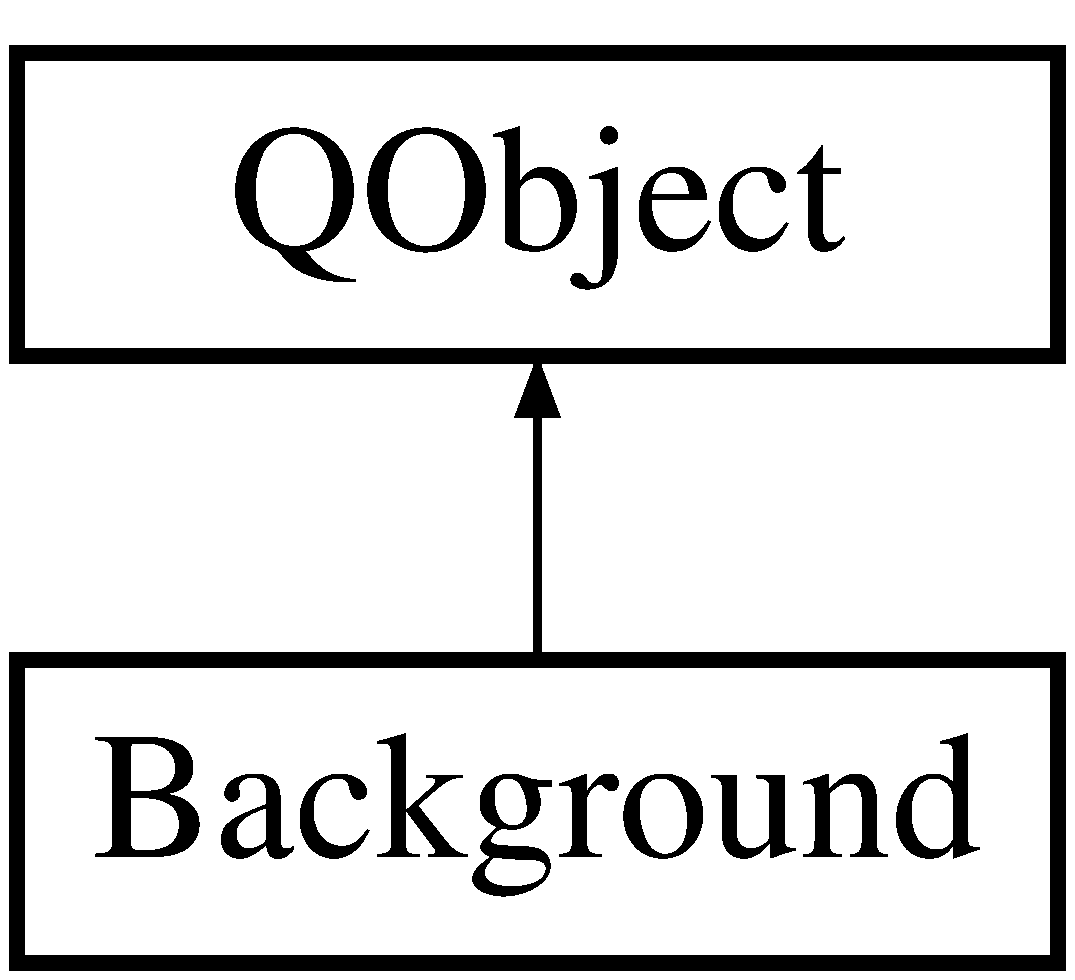
\includegraphics[height=2.000000cm]{class_background}
\end{center}
\end{figure}
\subsection*{Public Slots}
\begin{DoxyCompactItemize}
\item 
void \hyperlink{class_background_a57a08d996f7dd00395078adaf71cb223}{draw\+Background} (Q\+Painter $\ast$p)
\begin{DoxyCompactList}\small\item\em Zeichnet des Hintergrund. \end{DoxyCompactList}\end{DoxyCompactItemize}
\subsection*{Public Member Functions}
\begin{DoxyCompactItemize}
\item 
\hyperlink{class_background_ae3a96452f46575f9a43cecd172a26567}{Background} (int \+\_\+option, Q\+Object $\ast$parent=0)
\begin{DoxyCompactList}\small\item\em Constructor welcher die Images initialisiert. \end{DoxyCompactList}\end{DoxyCompactItemize}


\subsection{Detailed Description}
\hyperlink{class_background}{Background} Klasse für den Hintergrund. 

Diese Klasse stellt verschiedene Hintergründe für die verschiedenen Szenen zur Verfügung. 

\subsection{Constructor \& Destructor Documentation}
\hypertarget{class_background_ae3a96452f46575f9a43cecd172a26567}{}\index{Background@{Background}!Background@{Background}}
\index{Background@{Background}!Background@{Background}}
\subsubsection[{Background}]{\setlength{\rightskip}{0pt plus 5cm}Background\+::\+Background (
\begin{DoxyParamCaption}
\item[{int}]{\+\_\+option, }
\item[{Q\+Object $\ast$}]{parent = {\ttfamily 0}}
\end{DoxyParamCaption}
)\hspace{0.3cm}{\ttfamily [explicit]}}\label{class_background_ae3a96452f46575f9a43cecd172a26567}


Constructor welcher die Images initialisiert. 

Contructor der Klasse \hyperlink{class_background}{Background}. 
\begin{DoxyParams}{Parameters}
{\em \+\_\+option} & Gibt an welcher Hintergrund gewählt wird. \\
\hline
{\em parent} & Übergibt falls vorhanden das parent-\/\+Q\+Widget. \\
\hline
\end{DoxyParams}


\subsection{Member Function Documentation}
\hypertarget{class_background_a57a08d996f7dd00395078adaf71cb223}{}\index{Background@{Background}!draw\+Background@{draw\+Background}}
\index{draw\+Background@{draw\+Background}!Background@{Background}}
\subsubsection[{draw\+Background}]{\setlength{\rightskip}{0pt plus 5cm}void Background\+::draw\+Background (
\begin{DoxyParamCaption}
\item[{Q\+Painter $\ast$}]{p}
\end{DoxyParamCaption}
)\hspace{0.3cm}{\ttfamily [slot]}}\label{class_background_a57a08d996f7dd00395078adaf71cb223}


Zeichnet des Hintergrund. 

draw\+Background zeichnet den Hintergrund. 
\begin{DoxyParams}{Parameters}
{\em p} & Der Q\+Painter wird übergeben damit gezeichnet werden kann. \\
\hline
\end{DoxyParams}


The documentation for this class was generated from the following files\+:\begin{DoxyCompactItemize}
\item 
background.\+h\item 
background.\+cpp\end{DoxyCompactItemize}

\hypertarget{class_character}{}\section{Character Class Reference}
\label{class_character}\index{Character@{Character}}


\hyperlink{class_character}{Character} Klasse ist für die Darstellung und Bewegungen der Charaktere zuständig.  




{\ttfamily \#include $<$character.\+h$>$}

Inheritance diagram for Character\+:\begin{figure}[H]
\begin{center}
\leavevmode
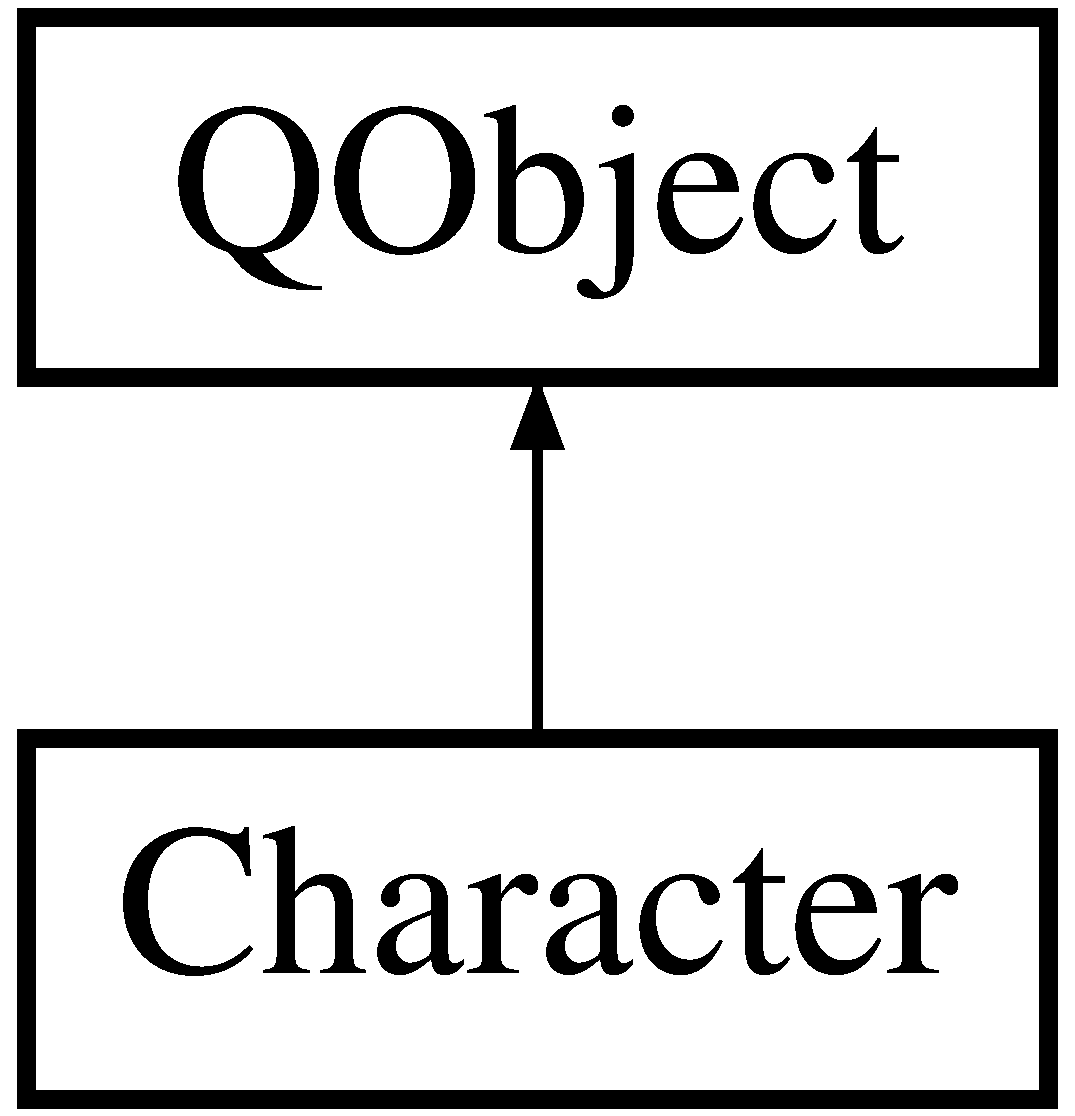
\includegraphics[height=2.000000cm]{class_character}
\end{center}
\end{figure}
\subsection*{Public Slots}
\begin{DoxyCompactItemize}
\item 
void \hyperlink{class_character_a732ddad97c8e4b271aac67ba1d7d3c98}{move\+Right} (bool value)
\begin{DoxyCompactList}\small\item\em Signalisiert das der Charakter nach rechts läuft oder nicht. \end{DoxyCompactList}\item 
void \hyperlink{class_character_adcc18bee13545c734c695dee06a9f094}{move\+Left} (bool value)
\begin{DoxyCompactList}\small\item\em Signalisiert das der Charakter nach links läuft oder nicht. \end{DoxyCompactList}\item 
void \hyperlink{class_character_a2257c559f50f1e78eea8d49dbe12af49}{jump\+Up} ()
\begin{DoxyCompactList}\small\item\em Signalisiert das der Charakter springt. \end{DoxyCompactList}\item 
void \hyperlink{class_character_a8cfbb3e6ea62013a74f7b837054ee03f}{set\+Crouch} (bool value)
\begin{DoxyCompactList}\small\item\em Signalisiert das der Charakter sich duckt oder sich nicht duckt. \end{DoxyCompactList}\item 
void \hyperlink{class_character_a5745dbf38bf7b408f254408f898a2e46}{punch} ()
\begin{DoxyCompactList}\small\item\em Signalisiert das der Charakter zuschlägt. \end{DoxyCompactList}\item 
void \hyperlink{class_character_aacbdc7590f8a9f6b295117a9675e2ab5}{reduce\+Life} (int redu)
\begin{DoxyCompactList}\small\item\em Verringert das Leben des Charakteres. \end{DoxyCompactList}\item 
void \hyperlink{class_character_a6a3f9b96fd22d73660f458e52a2e04ba}{set\+Life} (int value)
\begin{DoxyCompactList}\small\item\em Setzt das Leben eines Charakteres. \end{DoxyCompactList}\item 
void \hyperlink{class_character_a374c40a183c8c1795b10004a07b36fd7}{set\+Stunned} (bool value)
\begin{DoxyCompactList}\small\item\em Setzt den Charakter auf stunned oder nicht. \end{DoxyCompactList}\item 
bool \hyperlink{class_character_a2960bf6a336ffdfac0d19d0909ceb1dd}{enemy\+Is\+Left} (\hyperlink{class_character}{Character} $\ast$enemy)
\begin{DoxyCompactList}\small\item\em Gibt an ob ein Gegner sich links von einem befindet. \end{DoxyCompactList}\item 
bool \hyperlink{class_character_aea3908941f3be893dc1964b224e74825}{enemy\+Is\+Right} (\hyperlink{class_character}{Character} $\ast$enemy)
\begin{DoxyCompactList}\small\item\em Gibt an ob ein Gegner sich rechts von einem befindet. \end{DoxyCompactList}\item 
bool \hyperlink{class_character_aa4848867a1029966d670d5f492301308}{enemy\+Is\+Left\+Range} (\hyperlink{class_character}{Character} $\ast$enemy)
\begin{DoxyCompactList}\small\item\em Gibt an ob ein Gegner sich links und in schlagweite von einem befindet. \end{DoxyCompactList}\item 
bool \hyperlink{class_character_a6ae029174982ef952b074097789db3a4}{enemy\+Is\+Right\+Range} (\hyperlink{class_character}{Character} $\ast$enemy)
\begin{DoxyCompactList}\small\item\em Gibt an ob ein Gegner sich rechts und in schlagweite von einem befindet. \end{DoxyCompactList}\end{DoxyCompactItemize}
\subsection*{Signals}
\begin{DoxyCompactItemize}
\item 
void \hyperlink{class_character_a127f5ee58b01289418cf080a8328b6c7}{death} ()
\begin{DoxyCompactList}\small\item\em Der Charakter stirbt. \end{DoxyCompactList}\end{DoxyCompactItemize}
\subsection*{Public Member Functions}
\begin{DoxyCompactItemize}
\item 
\hyperlink{class_character_aefeb2b4e6d072de60e7cacb4d2c81b7a}{Character} (int \+\_\+option=1, bool enemy=false, Q\+Object $\ast$parent=0)
\begin{DoxyCompactList}\small\item\em Construktor der Klasse \hyperlink{class_character}{Character}. \end{DoxyCompactList}\item 
void \hyperlink{class_character_a876cf4bd6f6241810cb3f6072e8205ed}{draw\+Char} (Q\+Painter $\ast$p, \hyperlink{class_character}{Character} $\ast$e=N\+U\+L\+L)
\begin{DoxyCompactList}\small\item\em Zeichnet den Charakter. \end{DoxyCompactList}\item 
int \hyperlink{class_character_a4b4280b04c7b8839ffb46bb3be4cb490}{get\+X} ()
\begin{DoxyCompactList}\small\item\em Gibt den aktuellen X-\/\+Wert zurück den der Charakter hat. \end{DoxyCompactList}\item 
int \hyperlink{class_character_a28c072ac846a33336cc7c5fb869c4cd8}{get\+Y} ()
\begin{DoxyCompactList}\small\item\em Gibt den aktuellen Y-\/\+Wert zurück den der Charakter hat. \end{DoxyCompactList}\item 
int \hyperlink{class_character_a1e00eede43aa9b436b0cbd2127ab251a}{get\+Life} ()
\begin{DoxyCompactList}\small\item\em Gibt das aktuelle Leben des Charakteres zurück. \end{DoxyCompactList}\item 
int \hyperlink{class_character_a047f58799c51258670497cda68ca4b8c}{get\+Mana} ()
\begin{DoxyCompactList}\small\item\em Gibt das aktuelle Mana des Charakteres zurück. \end{DoxyCompactList}\item 
Q\+Image \hyperlink{class_character_abd97793fd7945f52850018713e7726e3}{get\+Icon} ()
\begin{DoxyCompactList}\small\item\em Gibt das Icon zurück als Q\+Image welches den Charakter darstellt. \end{DoxyCompactList}\item 
Q\+String \hyperlink{class_character_a2c4dcc76fbba8481fba7e175378a4cd0}{get\+Name} ()
\begin{DoxyCompactList}\small\item\em Gibt den Namen des aktuellen Charakteres zurück. \end{DoxyCompactList}\end{DoxyCompactItemize}


\subsection{Detailed Description}
\hyperlink{class_character}{Character} Klasse ist für die Darstellung und Bewegungen der Charaktere zuständig. 

Diese Klasse ist vollständig für das Zeichnen und Bewegen des Charakters zuständig. Sie wird von Draw.\+cpp aufgerufen. Um neue Bilder einzufügen muss nur im Contructer ein Case hinzugefügt werden, z.\+B. Case 2. Nun kann dann im Auswahlmenu für Charaktere die 2 gewählt werden (Mitte oben) und die Bilder dieses Charakteres werden geladen. Achte darauf alle Bilder, und auch auf die richtige größe eingefügt zu haben. Sonst wird es nicht funktionieren. Shadow kann so geladen werden wie er ist, er wird für alle Charaktere benutzt. 

\subsection{Constructor \& Destructor Documentation}
\hypertarget{class_character_aefeb2b4e6d072de60e7cacb4d2c81b7a}{}\index{Character@{Character}!Character@{Character}}
\index{Character@{Character}!Character@{Character}}
\subsubsection[{Character}]{\setlength{\rightskip}{0pt plus 5cm}Character\+::\+Character (
\begin{DoxyParamCaption}
\item[{int}]{\+\_\+option = {\ttfamily 1}, }
\item[{bool}]{enemy = {\ttfamily false}, }
\item[{Q\+Object $\ast$}]{parent = {\ttfamily 0}}
\end{DoxyParamCaption}
)\hspace{0.3cm}{\ttfamily [explicit]}}\label{class_character_aefeb2b4e6d072de60e7cacb4d2c81b7a}


Construktor der Klasse \hyperlink{class_character}{Character}. 

\hyperlink{class_character}{Character} 
\begin{DoxyParams}{Parameters}
{\em \+\_\+option} & Welcher Charakter ausgewählt wurde. \\
\hline
{\em enemy} & Ob ein Gegner existiert oder nicht (Computergegner). \\
\hline
{\em parent} & Das Parent Widget falls vorhanden. \\
\hline
\end{DoxyParams}


\subsection{Member Function Documentation}
\hypertarget{class_character_a127f5ee58b01289418cf080a8328b6c7}{}\index{Character@{Character}!death@{death}}
\index{death@{death}!Character@{Character}}
\subsubsection[{death}]{\setlength{\rightskip}{0pt plus 5cm}void Character\+::death (
\begin{DoxyParamCaption}
{}
\end{DoxyParamCaption}
)\hspace{0.3cm}{\ttfamily [signal]}}\label{class_character_a127f5ee58b01289418cf080a8328b6c7}


Der Charakter stirbt. 

death Signalisiert den Tod des aktuellen Charakteres. \hypertarget{class_character_a876cf4bd6f6241810cb3f6072e8205ed}{}\index{Character@{Character}!draw\+Char@{draw\+Char}}
\index{draw\+Char@{draw\+Char}!Character@{Character}}
\subsubsection[{draw\+Char}]{\setlength{\rightskip}{0pt plus 5cm}void Character\+::draw\+Char (
\begin{DoxyParamCaption}
\item[{Q\+Painter $\ast$}]{p, }
\item[{{\bf Character} $\ast$}]{e = {\ttfamily NULL}}
\end{DoxyParamCaption}
)}\label{class_character_a876cf4bd6f6241810cb3f6072e8205ed}


Zeichnet den Charakter. 

draw\+Char 
\begin{DoxyParams}{Parameters}
{\em p} & Der Painter damit gezeichnet werden kann. \\
\hline
{\em e} & Der Gegner falls vorhanden. \\
\hline
\end{DoxyParams}
\hypertarget{class_character_a2960bf6a336ffdfac0d19d0909ceb1dd}{}\index{Character@{Character}!enemy\+Is\+Left@{enemy\+Is\+Left}}
\index{enemy\+Is\+Left@{enemy\+Is\+Left}!Character@{Character}}
\subsubsection[{enemy\+Is\+Left}]{\setlength{\rightskip}{0pt plus 5cm}bool Character\+::enemy\+Is\+Left (
\begin{DoxyParamCaption}
\item[{{\bf Character} $\ast$}]{enemy}
\end{DoxyParamCaption}
)\hspace{0.3cm}{\ttfamily [slot]}}\label{class_character_a2960bf6a336ffdfac0d19d0909ceb1dd}


Gibt an ob ein Gegner sich links von einem befindet. 

enemy\+Is\+Left 
\begin{DoxyParams}{Parameters}
{\em enemy} & Variable der Klasse \hyperlink{class_character}{Character}, dies ist der Gegner. \\
\hline
\end{DoxyParams}
\begin{DoxyReturn}{Returns}
True -\/ Wenn der Gegner sich links befindet.~\newline
False -\/ Wenn nicht. 
\end{DoxyReturn}
\hypertarget{class_character_aa4848867a1029966d670d5f492301308}{}\index{Character@{Character}!enemy\+Is\+Left\+Range@{enemy\+Is\+Left\+Range}}
\index{enemy\+Is\+Left\+Range@{enemy\+Is\+Left\+Range}!Character@{Character}}
\subsubsection[{enemy\+Is\+Left\+Range}]{\setlength{\rightskip}{0pt plus 5cm}bool Character\+::enemy\+Is\+Left\+Range (
\begin{DoxyParamCaption}
\item[{{\bf Character} $\ast$}]{enemy}
\end{DoxyParamCaption}
)\hspace{0.3cm}{\ttfamily [slot]}}\label{class_character_aa4848867a1029966d670d5f492301308}


Gibt an ob ein Gegner sich links und in schlagweite von einem befindet. 

enemy\+Is\+Left\+Range 
\begin{DoxyParams}{Parameters}
{\em enemy} & Variable der Klasse \hyperlink{class_character}{Character}, dies ist der Gegner. \\
\hline
\end{DoxyParams}
\begin{DoxyReturn}{Returns}
True -\/ Wenn der Gegner sich links befindet und in schlagweite ist.~\newline
False -\/ Wenn nicht. 
\end{DoxyReturn}
\hypertarget{class_character_aea3908941f3be893dc1964b224e74825}{}\index{Character@{Character}!enemy\+Is\+Right@{enemy\+Is\+Right}}
\index{enemy\+Is\+Right@{enemy\+Is\+Right}!Character@{Character}}
\subsubsection[{enemy\+Is\+Right}]{\setlength{\rightskip}{0pt plus 5cm}bool Character\+::enemy\+Is\+Right (
\begin{DoxyParamCaption}
\item[{{\bf Character} $\ast$}]{enemy}
\end{DoxyParamCaption}
)\hspace{0.3cm}{\ttfamily [slot]}}\label{class_character_aea3908941f3be893dc1964b224e74825}


Gibt an ob ein Gegner sich rechts von einem befindet. 

enemy\+Is\+Right 
\begin{DoxyParams}{Parameters}
{\em enemy} & Variable der Klasse \hyperlink{class_character}{Character}, dies ist der Gegner. \\
\hline
\end{DoxyParams}
\begin{DoxyReturn}{Returns}
True -\/ Wenn der Gegner sich rechts befindet.~\newline
False -\/ Wenn nicht. 
\end{DoxyReturn}
\hypertarget{class_character_a6ae029174982ef952b074097789db3a4}{}\index{Character@{Character}!enemy\+Is\+Right\+Range@{enemy\+Is\+Right\+Range}}
\index{enemy\+Is\+Right\+Range@{enemy\+Is\+Right\+Range}!Character@{Character}}
\subsubsection[{enemy\+Is\+Right\+Range}]{\setlength{\rightskip}{0pt plus 5cm}bool Character\+::enemy\+Is\+Right\+Range (
\begin{DoxyParamCaption}
\item[{{\bf Character} $\ast$}]{enemy}
\end{DoxyParamCaption}
)\hspace{0.3cm}{\ttfamily [slot]}}\label{class_character_a6ae029174982ef952b074097789db3a4}


Gibt an ob ein Gegner sich rechts und in schlagweite von einem befindet. 

enemy\+Is\+Right\+Range 
\begin{DoxyParams}{Parameters}
{\em enemy} & Variable der Klasse \hyperlink{class_character}{Character}, dies ist der Gegner. \\
\hline
\end{DoxyParams}
\begin{DoxyReturn}{Returns}
True -\/ Wenn der Gegner sich rechts befindet und in schlagweite ist.~\newline
False -\/ Wenn nicht. 
\end{DoxyReturn}
\hypertarget{class_character_abd97793fd7945f52850018713e7726e3}{}\index{Character@{Character}!get\+Icon@{get\+Icon}}
\index{get\+Icon@{get\+Icon}!Character@{Character}}
\subsubsection[{get\+Icon}]{\setlength{\rightskip}{0pt plus 5cm}Q\+Image Character\+::get\+Icon (
\begin{DoxyParamCaption}
{}
\end{DoxyParamCaption}
)}\label{class_character_abd97793fd7945f52850018713e7726e3}


Gibt das Icon zurück als Q\+Image welches den Charakter darstellt. 

get\+Icon \begin{DoxyReturn}{Returns}
Icon von dem ausgewählten Charakter (Das Gesicht als Q\+Image). 
\end{DoxyReturn}
\hypertarget{class_character_a1e00eede43aa9b436b0cbd2127ab251a}{}\index{Character@{Character}!get\+Life@{get\+Life}}
\index{get\+Life@{get\+Life}!Character@{Character}}
\subsubsection[{get\+Life}]{\setlength{\rightskip}{0pt plus 5cm}int Character\+::get\+Life (
\begin{DoxyParamCaption}
{}
\end{DoxyParamCaption}
)}\label{class_character_a1e00eede43aa9b436b0cbd2127ab251a}


Gibt das aktuelle Leben des Charakteres zurück. 

get\+Life \begin{DoxyReturn}{Returns}
Der aktuelle Lebens-\/\+Wert des Charakteres. 
\end{DoxyReturn}
\hypertarget{class_character_a047f58799c51258670497cda68ca4b8c}{}\index{Character@{Character}!get\+Mana@{get\+Mana}}
\index{get\+Mana@{get\+Mana}!Character@{Character}}
\subsubsection[{get\+Mana}]{\setlength{\rightskip}{0pt plus 5cm}int Character\+::get\+Mana (
\begin{DoxyParamCaption}
{}
\end{DoxyParamCaption}
)}\label{class_character_a047f58799c51258670497cda68ca4b8c}


Gibt das aktuelle Mana des Charakteres zurück. 

get\+Mana \begin{DoxyReturn}{Returns}
Der aktuelle Mana-\/\+Wert des Charakteres. 
\end{DoxyReturn}
\hypertarget{class_character_a2c4dcc76fbba8481fba7e175378a4cd0}{}\index{Character@{Character}!get\+Name@{get\+Name}}
\index{get\+Name@{get\+Name}!Character@{Character}}
\subsubsection[{get\+Name}]{\setlength{\rightskip}{0pt plus 5cm}Q\+String Character\+::get\+Name (
\begin{DoxyParamCaption}
{}
\end{DoxyParamCaption}
)}\label{class_character_a2c4dcc76fbba8481fba7e175378a4cd0}


Gibt den Namen des aktuellen Charakteres zurück. 

get\+Name \begin{DoxyReturn}{Returns}
Name des aktuellen Charakteres. 
\end{DoxyReturn}
\hypertarget{class_character_a4b4280b04c7b8839ffb46bb3be4cb490}{}\index{Character@{Character}!get\+X@{get\+X}}
\index{get\+X@{get\+X}!Character@{Character}}
\subsubsection[{get\+X}]{\setlength{\rightskip}{0pt plus 5cm}int Character\+::get\+X (
\begin{DoxyParamCaption}
{}
\end{DoxyParamCaption}
)}\label{class_character_a4b4280b04c7b8839ffb46bb3be4cb490}


Gibt den aktuellen X-\/\+Wert zurück den der Charakter hat. 

get\+X \begin{DoxyReturn}{Returns}
Die aktuelle X-\/\+Position. 
\end{DoxyReturn}
\hypertarget{class_character_a28c072ac846a33336cc7c5fb869c4cd8}{}\index{Character@{Character}!get\+Y@{get\+Y}}
\index{get\+Y@{get\+Y}!Character@{Character}}
\subsubsection[{get\+Y}]{\setlength{\rightskip}{0pt plus 5cm}int Character\+::get\+Y (
\begin{DoxyParamCaption}
{}
\end{DoxyParamCaption}
)}\label{class_character_a28c072ac846a33336cc7c5fb869c4cd8}


Gibt den aktuellen Y-\/\+Wert zurück den der Charakter hat. 

get\+Y \begin{DoxyReturn}{Returns}
Die aktuelle Y-\/\+Position. 
\end{DoxyReturn}
\hypertarget{class_character_a2257c559f50f1e78eea8d49dbe12af49}{}\index{Character@{Character}!jump\+Up@{jump\+Up}}
\index{jump\+Up@{jump\+Up}!Character@{Character}}
\subsubsection[{jump\+Up}]{\setlength{\rightskip}{0pt plus 5cm}void Character\+::jump\+Up (
\begin{DoxyParamCaption}
{}
\end{DoxyParamCaption}
)\hspace{0.3cm}{\ttfamily [slot]}}\label{class_character_a2257c559f50f1e78eea8d49dbe12af49}


Signalisiert das der Charakter springt. 

jump\+Up \hypertarget{class_character_adcc18bee13545c734c695dee06a9f094}{}\index{Character@{Character}!move\+Left@{move\+Left}}
\index{move\+Left@{move\+Left}!Character@{Character}}
\subsubsection[{move\+Left}]{\setlength{\rightskip}{0pt plus 5cm}void Character\+::move\+Left (
\begin{DoxyParamCaption}
\item[{bool}]{value}
\end{DoxyParamCaption}
)\hspace{0.3cm}{\ttfamily [slot]}}\label{class_character_adcc18bee13545c734c695dee06a9f094}


Signalisiert das der Charakter nach links läuft oder nicht. 

move\+Left 
\begin{DoxyParams}{Parameters}
{\em value} & True -\/ läuft nach links.~\newline
False -\/ läuft nicht nach links. \\
\hline
\end{DoxyParams}
\hypertarget{class_character_a732ddad97c8e4b271aac67ba1d7d3c98}{}\index{Character@{Character}!move\+Right@{move\+Right}}
\index{move\+Right@{move\+Right}!Character@{Character}}
\subsubsection[{move\+Right}]{\setlength{\rightskip}{0pt plus 5cm}void Character\+::move\+Right (
\begin{DoxyParamCaption}
\item[{bool}]{value}
\end{DoxyParamCaption}
)\hspace{0.3cm}{\ttfamily [slot]}}\label{class_character_a732ddad97c8e4b271aac67ba1d7d3c98}


Signalisiert das der Charakter nach rechts läuft oder nicht. 

move\+Right 
\begin{DoxyParams}{Parameters}
{\em value} & True -\/ läuft nach rechts.~\newline
False -\/ läuft nicht nach rechts. \\
\hline
\end{DoxyParams}
\hypertarget{class_character_a5745dbf38bf7b408f254408f898a2e46}{}\index{Character@{Character}!punch@{punch}}
\index{punch@{punch}!Character@{Character}}
\subsubsection[{punch}]{\setlength{\rightskip}{0pt plus 5cm}void Character\+::punch (
\begin{DoxyParamCaption}
{}
\end{DoxyParamCaption}
)\hspace{0.3cm}{\ttfamily [slot]}}\label{class_character_a5745dbf38bf7b408f254408f898a2e46}


Signalisiert das der Charakter zuschlägt. 

punch \hypertarget{class_character_aacbdc7590f8a9f6b295117a9675e2ab5}{}\index{Character@{Character}!reduce\+Life@{reduce\+Life}}
\index{reduce\+Life@{reduce\+Life}!Character@{Character}}
\subsubsection[{reduce\+Life}]{\setlength{\rightskip}{0pt plus 5cm}void Character\+::reduce\+Life (
\begin{DoxyParamCaption}
\item[{int}]{redu}
\end{DoxyParamCaption}
)\hspace{0.3cm}{\ttfamily [slot]}}\label{class_character_aacbdc7590f8a9f6b295117a9675e2ab5}


Verringert das Leben des Charakteres. 

reduce\+Life 
\begin{DoxyParams}{Parameters}
{\em redu} & Die Menge um wieviel es reduziert wird. \\
\hline
\end{DoxyParams}
\hypertarget{class_character_a8cfbb3e6ea62013a74f7b837054ee03f}{}\index{Character@{Character}!set\+Crouch@{set\+Crouch}}
\index{set\+Crouch@{set\+Crouch}!Character@{Character}}
\subsubsection[{set\+Crouch}]{\setlength{\rightskip}{0pt plus 5cm}void Character\+::set\+Crouch (
\begin{DoxyParamCaption}
\item[{bool}]{value}
\end{DoxyParamCaption}
)\hspace{0.3cm}{\ttfamily [slot]}}\label{class_character_a8cfbb3e6ea62013a74f7b837054ee03f}


Signalisiert das der Charakter sich duckt oder sich nicht duckt. 

set\+Crouch 
\begin{DoxyParams}{Parameters}
{\em value} & True -\/ der Charaktere duckt sich.~\newline
False -\/ der Charaktere duckt sich nicht. \\
\hline
\end{DoxyParams}
\hypertarget{class_character_a6a3f9b96fd22d73660f458e52a2e04ba}{}\index{Character@{Character}!set\+Life@{set\+Life}}
\index{set\+Life@{set\+Life}!Character@{Character}}
\subsubsection[{set\+Life}]{\setlength{\rightskip}{0pt plus 5cm}void Character\+::set\+Life (
\begin{DoxyParamCaption}
\item[{int}]{value}
\end{DoxyParamCaption}
)\hspace{0.3cm}{\ttfamily [slot]}}\label{class_character_a6a3f9b96fd22d73660f458e52a2e04ba}


Setzt das Leben eines Charakteres. 

set\+Life 
\begin{DoxyParams}{Parameters}
{\em value} & Die Menge des Lebens das gesetzt werden soll. \\
\hline
\end{DoxyParams}
\hypertarget{class_character_a374c40a183c8c1795b10004a07b36fd7}{}\index{Character@{Character}!set\+Stunned@{set\+Stunned}}
\index{set\+Stunned@{set\+Stunned}!Character@{Character}}
\subsubsection[{set\+Stunned}]{\setlength{\rightskip}{0pt plus 5cm}void Character\+::set\+Stunned (
\begin{DoxyParamCaption}
\item[{bool}]{value}
\end{DoxyParamCaption}
)\hspace{0.3cm}{\ttfamily [slot]}}\label{class_character_a374c40a183c8c1795b10004a07b36fd7}


Setzt den Charakter auf stunned oder nicht. 

set\+Stunned 
\begin{DoxyParams}{Parameters}
{\em value} & True -\/ Charakter ist stunned.~\newline
False -\/ Charakter ist nicht stunned. \\
\hline
\end{DoxyParams}


The documentation for this class was generated from the following files\+:\begin{DoxyCompactItemize}
\item 
character.\+h\item 
character.\+cpp\end{DoxyCompactItemize}

\hypertarget{class_chat}{}\section{Chat Class Reference}
\label{class_chat}\index{Chat@{Chat}}


\hyperlink{class_chat}{Chat} Klasse beschäftigt sich damit einen \hyperlink{class_chat}{Chat} anzuzeigen und ihn auszuwerten.  




{\ttfamily \#include $<$chat.\+h$>$}

Inheritance diagram for Chat\+:\begin{figure}[H]
\begin{center}
\leavevmode
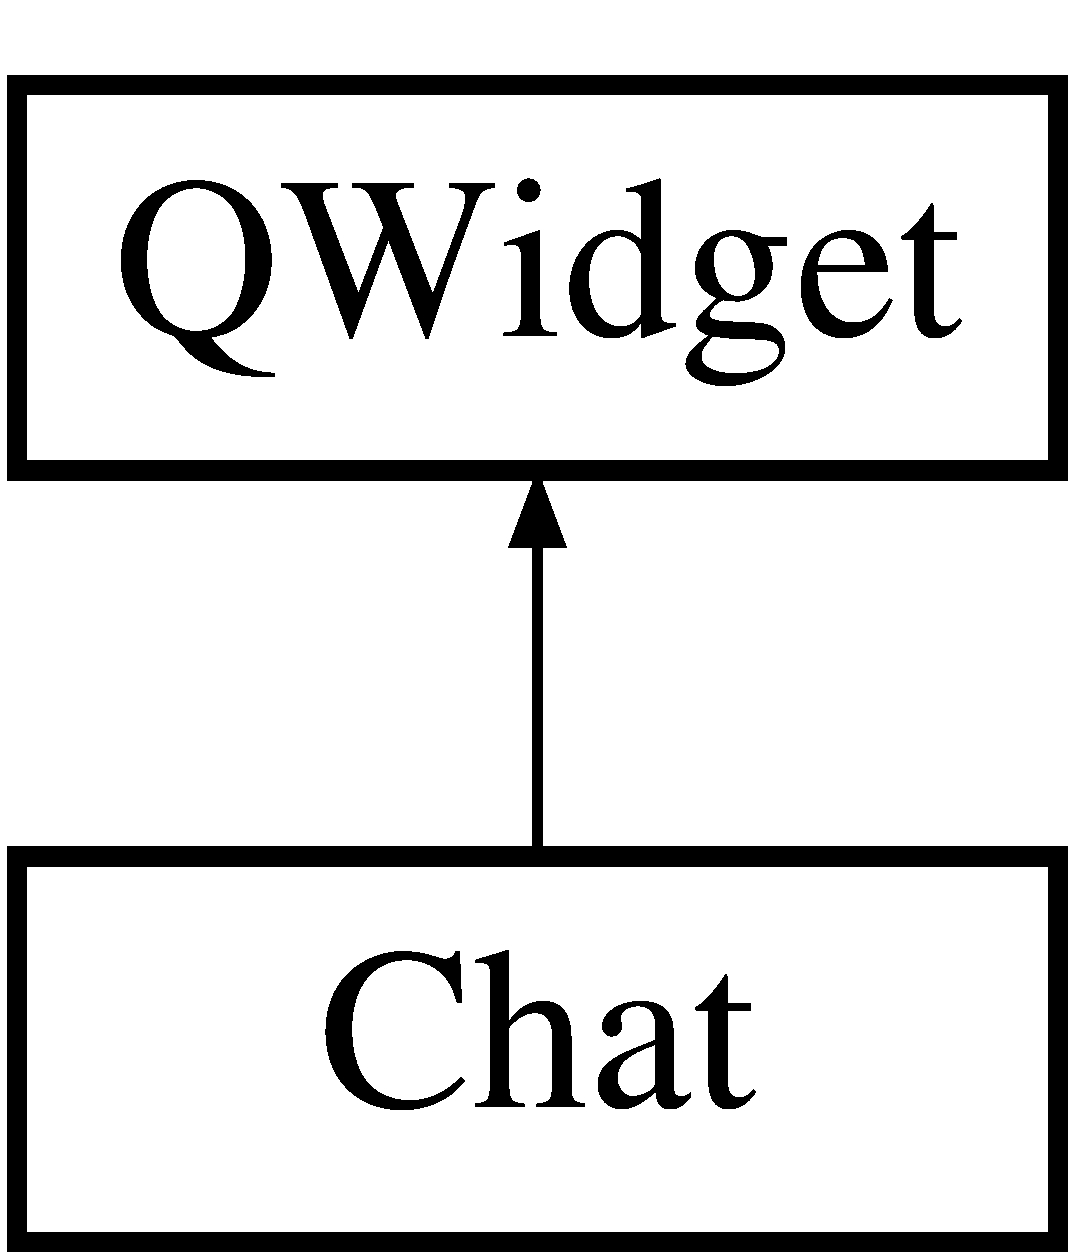
\includegraphics[height=2.000000cm]{class_chat}
\end{center}
\end{figure}
\subsection*{Public Slots}
\begin{DoxyCompactItemize}
\item 
void \hyperlink{class_chat_a7b94bde4d4e53034b558a0aa0b8b76eb}{signal} ()
\begin{DoxyCompactList}\small\item\em Signalisiert dem \hyperlink{class_chat}{Chat} das er versteckt oder angezeigt werden soll. \end{DoxyCompactList}\item 
void \hyperlink{class_chat_aac15e09ec782dcee4a6f98492aa10633}{show\+Only\+Chat} ()
\begin{DoxyCompactList}\small\item\em Zeigt nur den \hyperlink{class_chat}{Chat}. \end{DoxyCompactList}\item 
void \hyperlink{class_chat_a7da9c4b3521928b4c85efce819a2e2d5}{hide\+Only\+Chat} ()
\begin{DoxyCompactList}\small\item\em Versteckt nur den \hyperlink{class_chat}{Chat}. \end{DoxyCompactList}\end{DoxyCompactItemize}
\subsection*{Signals}
\begin{DoxyCompactItemize}
\item 
void \hyperlink{class_chat_a49a01e63da7824bbd162d253a059fad8}{set\+Current} (int a)
\begin{DoxyCompactList}\small\item\em Signalisiert der Main das ein anderes Widget angezeigt werden soll. \end{DoxyCompactList}\item 
void \hyperlink{class_chat_ac425c72f7a120ef313113083891a3966}{set\+Focus\+To} (int a)
\begin{DoxyCompactList}\small\item\em Signalisiert der Main das ein anderes Widget den Focus bekommen soll. \end{DoxyCompactList}\end{DoxyCompactItemize}
\subsection*{Public Member Functions}
\begin{DoxyCompactItemize}
\item 
\hyperlink{class_chat_a83c846c142bde1a2a96dd17eb6544f6f}{Chat} (Q\+Widget $\ast$parent=0)
\begin{DoxyCompactList}\small\item\em Contructor der Klasse \hyperlink{class_chat}{Chat}. \end{DoxyCompactList}\end{DoxyCompactItemize}


\subsection{Detailed Description}
\hyperlink{class_chat}{Chat} Klasse beschäftigt sich damit einen \hyperlink{class_chat}{Chat} anzuzeigen und ihn auszuwerten. 

\subsection{Constructor \& Destructor Documentation}
\hypertarget{class_chat_a83c846c142bde1a2a96dd17eb6544f6f}{}\index{Chat@{Chat}!Chat@{Chat}}
\index{Chat@{Chat}!Chat@{Chat}}
\subsubsection[{Chat}]{\setlength{\rightskip}{0pt plus 5cm}Chat\+::\+Chat (
\begin{DoxyParamCaption}
\item[{Q\+Widget $\ast$}]{parent = {\ttfamily 0}}
\end{DoxyParamCaption}
)\hspace{0.3cm}{\ttfamily [explicit]}}\label{class_chat_a83c846c142bde1a2a96dd17eb6544f6f}


Contructor der Klasse \hyperlink{class_chat}{Chat}. 

\hyperlink{class_chat}{Chat} Erstellt einige standardvariable für die Klasse. 
\begin{DoxyParams}{Parameters}
{\em parent} & Das parent Widget falls vorhanden. \\
\hline
\end{DoxyParams}


\subsection{Member Function Documentation}
\hypertarget{class_chat_a7da9c4b3521928b4c85efce819a2e2d5}{}\index{Chat@{Chat}!hide\+Only\+Chat@{hide\+Only\+Chat}}
\index{hide\+Only\+Chat@{hide\+Only\+Chat}!Chat@{Chat}}
\subsubsection[{hide\+Only\+Chat}]{\setlength{\rightskip}{0pt plus 5cm}void Chat\+::hide\+Only\+Chat (
\begin{DoxyParamCaption}
{}
\end{DoxyParamCaption}
)\hspace{0.3cm}{\ttfamily [slot]}}\label{class_chat_a7da9c4b3521928b4c85efce819a2e2d5}


Versteckt nur den \hyperlink{class_chat}{Chat}. 

hide\+Only\+Chat \hypertarget{class_chat_a49a01e63da7824bbd162d253a059fad8}{}\index{Chat@{Chat}!set\+Current@{set\+Current}}
\index{set\+Current@{set\+Current}!Chat@{Chat}}
\subsubsection[{set\+Current}]{\setlength{\rightskip}{0pt plus 5cm}void Chat\+::set\+Current (
\begin{DoxyParamCaption}
\item[{int}]{a}
\end{DoxyParamCaption}
)\hspace{0.3cm}{\ttfamily [signal]}}\label{class_chat_a49a01e63da7824bbd162d253a059fad8}


Signalisiert der Main das ein anderes Widget angezeigt werden soll. 

set\+Current 
\begin{DoxyParams}{Parameters}
{\em a} & Das Widget welches angezeigt werden soll. \\
\hline
\end{DoxyParams}
\hypertarget{class_chat_ac425c72f7a120ef313113083891a3966}{}\index{Chat@{Chat}!set\+Focus\+To@{set\+Focus\+To}}
\index{set\+Focus\+To@{set\+Focus\+To}!Chat@{Chat}}
\subsubsection[{set\+Focus\+To}]{\setlength{\rightskip}{0pt plus 5cm}void Chat\+::set\+Focus\+To (
\begin{DoxyParamCaption}
\item[{int}]{a}
\end{DoxyParamCaption}
)\hspace{0.3cm}{\ttfamily [signal]}}\label{class_chat_ac425c72f7a120ef313113083891a3966}


Signalisiert der Main das ein anderes Widget den Focus bekommen soll. 

set\+Focus\+To 
\begin{DoxyParams}{Parameters}
{\em a} & Das widget welches den Focus bekommen soll. \\
\hline
\end{DoxyParams}
\hypertarget{class_chat_aac15e09ec782dcee4a6f98492aa10633}{}\index{Chat@{Chat}!show\+Only\+Chat@{show\+Only\+Chat}}
\index{show\+Only\+Chat@{show\+Only\+Chat}!Chat@{Chat}}
\subsubsection[{show\+Only\+Chat}]{\setlength{\rightskip}{0pt plus 5cm}void Chat\+::show\+Only\+Chat (
\begin{DoxyParamCaption}
{}
\end{DoxyParamCaption}
)\hspace{0.3cm}{\ttfamily [slot]}}\label{class_chat_aac15e09ec782dcee4a6f98492aa10633}


Zeigt nur den \hyperlink{class_chat}{Chat}. 

show\+Only\+Chat \hypertarget{class_chat_a7b94bde4d4e53034b558a0aa0b8b76eb}{}\index{Chat@{Chat}!signal@{signal}}
\index{signal@{signal}!Chat@{Chat}}
\subsubsection[{signal}]{\setlength{\rightskip}{0pt plus 5cm}void Chat\+::signal (
\begin{DoxyParamCaption}
{}
\end{DoxyParamCaption}
)\hspace{0.3cm}{\ttfamily [slot]}}\label{class_chat_a7b94bde4d4e53034b558a0aa0b8b76eb}


Signalisiert dem \hyperlink{class_chat}{Chat} das er versteckt oder angezeigt werden soll. 

signal 

The documentation for this class was generated from the following files\+:\begin{DoxyCompactItemize}
\item 
chat.\+h\item 
chat.\+cpp\end{DoxyCompactItemize}

\hypertarget{class_choose_background}{}\section{Choose\+Background Class Reference}
\label{class_choose_background}\index{Choose\+Background@{Choose\+Background}}


choose\+Background Klasse symbolisiert ein Auswahlwidget in welchem der Benutzer einen Hintergrund für sein Spiel auswählen kann.  




{\ttfamily \#include $<$choosebackground.\+h$>$}

Inheritance diagram for Choose\+Background\+:\begin{figure}[H]
\begin{center}
\leavevmode
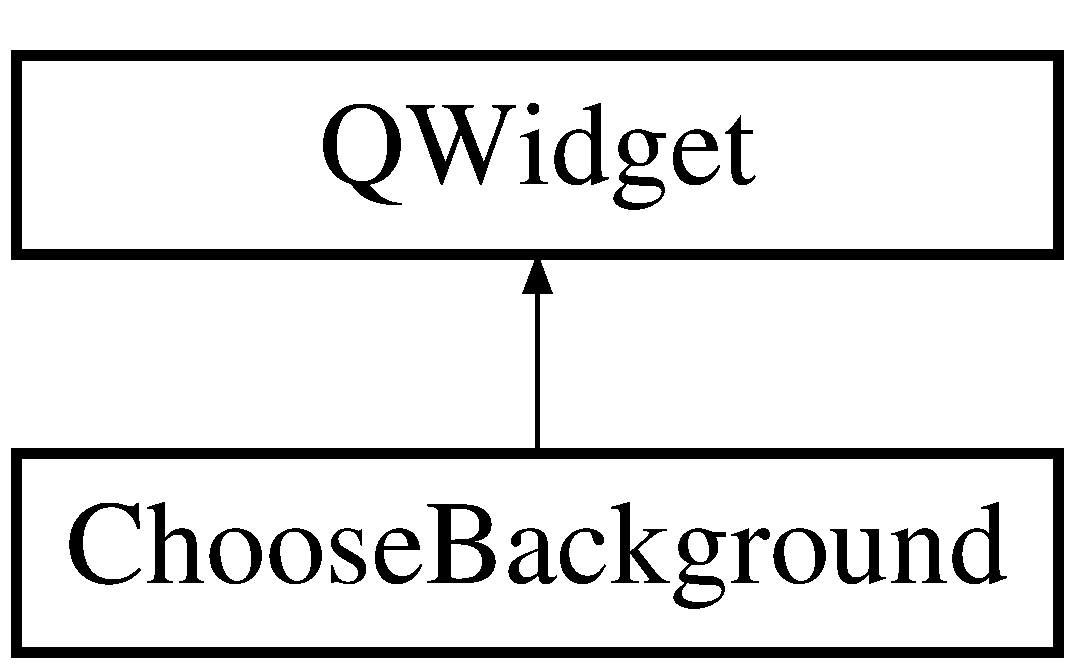
\includegraphics[height=2.000000cm]{class_choose_background}
\end{center}
\end{figure}
\subsection*{Public Slots}
\begin{DoxyCompactItemize}
\item 
\hypertarget{class_choose_background_a134632704516ff01d21147a6f7238b8f}{}void \hyperlink{class_choose_background_a134632704516ff01d21147a6f7238b8f}{selected\+Left} ()\label{class_choose_background_a134632704516ff01d21147a6f7238b8f}

\begin{DoxyCompactList}\small\item\em Wird angetriggert wenn das linke Icon selektiert wurde. \end{DoxyCompactList}\item 
\hypertarget{class_choose_background_a9fa9d22a3cfd437307117bb32036b731}{}void \hyperlink{class_choose_background_a9fa9d22a3cfd437307117bb32036b731}{selected\+Mid} ()\label{class_choose_background_a9fa9d22a3cfd437307117bb32036b731}

\begin{DoxyCompactList}\small\item\em Wird angetriggert wenn das mittige Icon selektiert wurde. \end{DoxyCompactList}\item 
\hypertarget{class_choose_background_afc6ef25b1b6e1ed1e9842be71542a092}{}void \hyperlink{class_choose_background_afc6ef25b1b6e1ed1e9842be71542a092}{selected\+Right} ()\label{class_choose_background_afc6ef25b1b6e1ed1e9842be71542a092}

\begin{DoxyCompactList}\small\item\em Wird angetriggert wenn das rechte Icon selektiert wurde. \end{DoxyCompactList}\end{DoxyCompactItemize}
\subsection*{Signals}
\begin{DoxyCompactItemize}
\item 
void \hyperlink{class_choose_background_afe5384a4f9751980654331f16f9880d6}{set\+Current} (int)
\begin{DoxyCompactList}\small\item\em Signalisiert der Main das ein anderes Widget angezeigt werden soll. \end{DoxyCompactList}\item 
void \hyperlink{class_choose_background_a97f62dc7c7f8c0311bcb4d9de40f8961}{set\+Background} (int)
\begin{DoxyCompactList}\small\item\em Signalisiert der Main das ein background ausgewählt wurde. \end{DoxyCompactList}\item 
void \hyperlink{class_choose_background_a60e09b439c577557e659a7c8cd17ef95}{right} ()
\begin{DoxyCompactList}\small\item\em Signalisiert das der Anweder nach rechts gegangen ist. \end{DoxyCompactList}\item 
void \hyperlink{class_choose_background_ad94244d54915e86b87745df492dab6e6}{left} ()
\begin{DoxyCompactList}\small\item\em Signalisiert das der Anweder nach links gegangen ist. \end{DoxyCompactList}\end{DoxyCompactItemize}
\subsection*{Public Member Functions}
\begin{DoxyCompactItemize}
\item 
\hyperlink{class_choose_background_ab7ee660174665e9bc68eb183817ca099}{Choose\+Background} (Q\+Widget $\ast$parent=0)
\begin{DoxyCompactList}\small\item\em Contructor der choose\+Background Klasse. \end{DoxyCompactList}\end{DoxyCompactItemize}
\subsection*{Protected Member Functions}
\begin{DoxyCompactItemize}
\item 
void \hyperlink{class_choose_background_a380e9e5f617b252967ac18726ad391d4}{paint\+Event} (Q\+Paint\+Event $\ast$e)
\begin{DoxyCompactList}\small\item\em Zeichnet Elemente für die Klasse. \end{DoxyCompactList}\item 
void \hyperlink{class_choose_background_a76473476547b89b1bd7712caafec5068}{key\+Press\+Event} (Q\+Key\+Event $\ast$e)
\begin{DoxyCompactList}\small\item\em Registriert die Tastenschläge des Benutzers. \end{DoxyCompactList}\end{DoxyCompactItemize}


\subsection{Detailed Description}
choose\+Background Klasse symbolisiert ein Auswahlwidget in welchem der Benutzer einen Hintergrund für sein Spiel auswählen kann. 

\subsection{Constructor \& Destructor Documentation}
\hypertarget{class_choose_background_ab7ee660174665e9bc68eb183817ca099}{}\index{Choose\+Background@{Choose\+Background}!Choose\+Background@{Choose\+Background}}
\index{Choose\+Background@{Choose\+Background}!Choose\+Background@{Choose\+Background}}
\subsubsection[{Choose\+Background}]{\setlength{\rightskip}{0pt plus 5cm}Choose\+Background\+::\+Choose\+Background (
\begin{DoxyParamCaption}
\item[{Q\+Widget $\ast$}]{parent = {\ttfamily 0}}
\end{DoxyParamCaption}
)\hspace{0.3cm}{\ttfamily [explicit]}}\label{class_choose_background_ab7ee660174665e9bc68eb183817ca099}


Contructor der choose\+Background Klasse. 

\hyperlink{class_choose_background}{Choose\+Background} Erstellt die nötigen Image dateien und initialisiert die Einstellungen für das Auswahlmenü. 
\begin{DoxyParams}{Parameters}
{\em parent} & Das parent Widget falls vorhanden. \\
\hline
\end{DoxyParams}


\subsection{Member Function Documentation}
\hypertarget{class_choose_background_a76473476547b89b1bd7712caafec5068}{}\index{Choose\+Background@{Choose\+Background}!key\+Press\+Event@{key\+Press\+Event}}
\index{key\+Press\+Event@{key\+Press\+Event}!Choose\+Background@{Choose\+Background}}
\subsubsection[{key\+Press\+Event}]{\setlength{\rightskip}{0pt plus 5cm}void Choose\+Background\+::key\+Press\+Event (
\begin{DoxyParamCaption}
\item[{Q\+Key\+Event $\ast$}]{e}
\end{DoxyParamCaption}
)\hspace{0.3cm}{\ttfamily [protected]}}\label{class_choose_background_a76473476547b89b1bd7712caafec5068}


Registriert die Tastenschläge des Benutzers. 

key\+Press\+Event 
\begin{DoxyParams}{Parameters}
{\em e} & Die Taste welche gedrückt wird. \\
\hline
\end{DoxyParams}
\hypertarget{class_choose_background_ad94244d54915e86b87745df492dab6e6}{}\index{Choose\+Background@{Choose\+Background}!left@{left}}
\index{left@{left}!Choose\+Background@{Choose\+Background}}
\subsubsection[{left}]{\setlength{\rightskip}{0pt plus 5cm}void Choose\+Background\+::left (
\begin{DoxyParamCaption}
{}
\end{DoxyParamCaption}
)\hspace{0.3cm}{\ttfamily [signal]}}\label{class_choose_background_ad94244d54915e86b87745df492dab6e6}


Signalisiert das der Anweder nach links gegangen ist. 

left \hypertarget{class_choose_background_a380e9e5f617b252967ac18726ad391d4}{}\index{Choose\+Background@{Choose\+Background}!paint\+Event@{paint\+Event}}
\index{paint\+Event@{paint\+Event}!Choose\+Background@{Choose\+Background}}
\subsubsection[{paint\+Event}]{\setlength{\rightskip}{0pt plus 5cm}void Choose\+Background\+::paint\+Event (
\begin{DoxyParamCaption}
\item[{Q\+Paint\+Event $\ast$}]{e}
\end{DoxyParamCaption}
)\hspace{0.3cm}{\ttfamily [protected]}}\label{class_choose_background_a380e9e5f617b252967ac18726ad391d4}


Zeichnet Elemente für die Klasse. 

paint\+Event 
\begin{DoxyParams}{Parameters}
{\em e} & Das paint\+Event. \\
\hline
\end{DoxyParams}
\hypertarget{class_choose_background_a60e09b439c577557e659a7c8cd17ef95}{}\index{Choose\+Background@{Choose\+Background}!right@{right}}
\index{right@{right}!Choose\+Background@{Choose\+Background}}
\subsubsection[{right}]{\setlength{\rightskip}{0pt plus 5cm}void Choose\+Background\+::right (
\begin{DoxyParamCaption}
{}
\end{DoxyParamCaption}
)\hspace{0.3cm}{\ttfamily [signal]}}\label{class_choose_background_a60e09b439c577557e659a7c8cd17ef95}


Signalisiert das der Anweder nach rechts gegangen ist. 

right \hypertarget{class_choose_background_a97f62dc7c7f8c0311bcb4d9de40f8961}{}\index{Choose\+Background@{Choose\+Background}!set\+Background@{set\+Background}}
\index{set\+Background@{set\+Background}!Choose\+Background@{Choose\+Background}}
\subsubsection[{set\+Background}]{\setlength{\rightskip}{0pt plus 5cm}void Choose\+Background\+::set\+Background (
\begin{DoxyParamCaption}
\item[{int}]{}
\end{DoxyParamCaption}
)\hspace{0.3cm}{\ttfamily [signal]}}\label{class_choose_background_a97f62dc7c7f8c0311bcb4d9de40f8961}


Signalisiert der Main das ein background ausgewählt wurde. 

set\+Background 
\begin{DoxyParams}{Parameters}
{\em Der} & background der ausgewählt wurde. \\
\hline
\end{DoxyParams}
\hypertarget{class_choose_background_afe5384a4f9751980654331f16f9880d6}{}\index{Choose\+Background@{Choose\+Background}!set\+Current@{set\+Current}}
\index{set\+Current@{set\+Current}!Choose\+Background@{Choose\+Background}}
\subsubsection[{set\+Current}]{\setlength{\rightskip}{0pt plus 5cm}void Choose\+Background\+::set\+Current (
\begin{DoxyParamCaption}
\item[{int}]{}
\end{DoxyParamCaption}
)\hspace{0.3cm}{\ttfamily [signal]}}\label{class_choose_background_afe5384a4f9751980654331f16f9880d6}


Signalisiert der Main das ein anderes Widget angezeigt werden soll. 

set\+Current 
\begin{DoxyParams}{Parameters}
{\em Das} & Widget welches angezeigt werden soll. \\
\hline
\end{DoxyParams}


The documentation for this class was generated from the following files\+:\begin{DoxyCompactItemize}
\item 
choosebackground.\+h\item 
choosebackground.\+cpp\end{DoxyCompactItemize}

\hypertarget{class_choose_menu}{}\section{Choose\+Menu Class Reference}
\label{class_choose_menu}\index{Choose\+Menu@{Choose\+Menu}}
Inheritance diagram for Choose\+Menu\+:\begin{figure}[H]
\begin{center}
\leavevmode
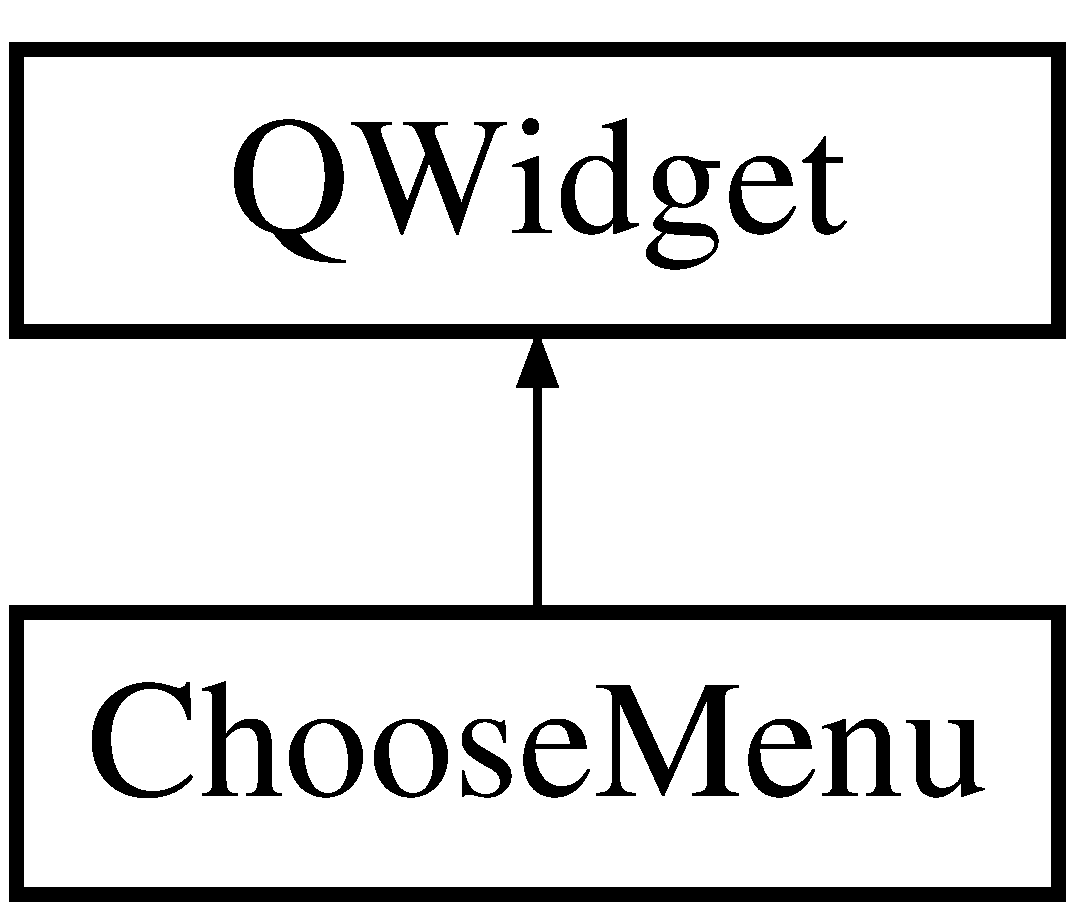
\includegraphics[height=2.000000cm]{class_choose_menu}
\end{center}
\end{figure}
\subsection*{Signals}
\begin{DoxyCompactItemize}
\item 
\hypertarget{class_choose_menu_a053dc4e1fccc670fd57940a9143ba70e}{}void {\bfseries set\+Current} (int)\label{class_choose_menu_a053dc4e1fccc670fd57940a9143ba70e}

\item 
\hypertarget{class_choose_menu_a9ddf26dbd1f7e26d80978de6a881ee1b}{}void {\bfseries set\+Character} (int)\label{class_choose_menu_a9ddf26dbd1f7e26d80978de6a881ee1b}

\item 
\hypertarget{class_choose_menu_af8b98075fd4c7c50ad7417852e8ed226}{}void {\bfseries set\+Character2} (int)\label{class_choose_menu_af8b98075fd4c7c50ad7417852e8ed226}

\item 
\hypertarget{class_choose_menu_ab60b2705eb02edf89244d2f44debd3e7}{}void {\bfseries right} ()\label{class_choose_menu_ab60b2705eb02edf89244d2f44debd3e7}

\item 
\hypertarget{class_choose_menu_a667b64a72cbadf598af6eadd27d474de}{}void {\bfseries down} ()\label{class_choose_menu_a667b64a72cbadf598af6eadd27d474de}

\item 
\hypertarget{class_choose_menu_aab43a0cf8d120937626a34f24ba29342}{}void {\bfseries up} ()\label{class_choose_menu_aab43a0cf8d120937626a34f24ba29342}

\item 
\hypertarget{class_choose_menu_a583409f96522df4268a0d3441380b492}{}void {\bfseries left} ()\label{class_choose_menu_a583409f96522df4268a0d3441380b492}

\end{DoxyCompactItemize}
\subsection*{Public Member Functions}
\begin{DoxyCompactItemize}
\item 
\hyperlink{class_choose_menu_ad44e7c05565bcea6c75ba6ddde2f0c51}{Choose\+Menu} (Q\+Widget $\ast$parent=0)
\begin{DoxyCompactList}\small\item\em \hyperlink{class_choose_menu_ad44e7c05565bcea6c75ba6ddde2f0c51}{Choose\+Menu\+::\+Choose\+Menu}. \end{DoxyCompactList}\item 
void \hyperlink{class_choose_menu_aa87f53c54f73ff60e7b4b3e77b2fa4b2}{set\+Player\+Vs\+Player} (bool value)
\begin{DoxyCompactList}\small\item\em \hyperlink{class_choose_menu_aa87f53c54f73ff60e7b4b3e77b2fa4b2}{Choose\+Menu\+::set\+Player\+Vs\+Player}. \end{DoxyCompactList}\end{DoxyCompactItemize}
\subsection*{Protected Member Functions}
\begin{DoxyCompactItemize}
\item 
void \hyperlink{class_choose_menu_a98996879611931da4a621b752ecdf4d1}{paint\+Event} (Q\+Paint\+Event $\ast$e)
\begin{DoxyCompactList}\small\item\em \hyperlink{class_choose_menu_a98996879611931da4a621b752ecdf4d1}{Choose\+Menu\+::paint\+Event}. \end{DoxyCompactList}\item 
void \hyperlink{class_choose_menu_ae3fec13ab674dc4a7b012efcc2b9c4f6}{key\+Press\+Event} (Q\+Key\+Event $\ast$e)
\begin{DoxyCompactList}\small\item\em \hyperlink{class_choose_menu_ae3fec13ab674dc4a7b012efcc2b9c4f6}{Choose\+Menu\+::key\+Press\+Event}. \end{DoxyCompactList}\item 
void \hyperlink{class_choose_menu_a89be0220a1eeb013ddc50ba27d4fa808}{key\+Release\+Event} (Q\+Key\+Event $\ast$e)
\begin{DoxyCompactList}\small\item\em \hyperlink{class_choose_menu_a89be0220a1eeb013ddc50ba27d4fa808}{Choose\+Menu\+::key\+Release\+Event}. \end{DoxyCompactList}\end{DoxyCompactItemize}


\subsection{Constructor \& Destructor Documentation}
\hypertarget{class_choose_menu_ad44e7c05565bcea6c75ba6ddde2f0c51}{}\index{Choose\+Menu@{Choose\+Menu}!Choose\+Menu@{Choose\+Menu}}
\index{Choose\+Menu@{Choose\+Menu}!Choose\+Menu@{Choose\+Menu}}
\subsubsection[{Choose\+Menu}]{\setlength{\rightskip}{0pt plus 5cm}Choose\+Menu\+::\+Choose\+Menu (
\begin{DoxyParamCaption}
\item[{Q\+Widget $\ast$}]{parent = {\ttfamily 0}}
\end{DoxyParamCaption}
)\hspace{0.3cm}{\ttfamily [explicit]}}\label{class_choose_menu_ad44e7c05565bcea6c75ba6ddde2f0c51}


\hyperlink{class_choose_menu_ad44e7c05565bcea6c75ba6ddde2f0c51}{Choose\+Menu\+::\+Choose\+Menu}. 

Diese Klasse repräsentiert die Charakterauswahl, sie zeigt die Charaktere an und fängt die Tasten ab die der Benutzer eingibt. Wenn der Benutzer fertig ist werden die Daten weitergegeben und es wird zur Hauptklasse zurückgekehrt.


\begin{DoxyParams}{Parameters}
{\em parent} & The parent widget. \\
\hline
\end{DoxyParams}


\subsection{Member Function Documentation}
\hypertarget{class_choose_menu_ae3fec13ab674dc4a7b012efcc2b9c4f6}{}\index{Choose\+Menu@{Choose\+Menu}!key\+Press\+Event@{key\+Press\+Event}}
\index{key\+Press\+Event@{key\+Press\+Event}!Choose\+Menu@{Choose\+Menu}}
\subsubsection[{key\+Press\+Event}]{\setlength{\rightskip}{0pt plus 5cm}void Choose\+Menu\+::key\+Press\+Event (
\begin{DoxyParamCaption}
\item[{Q\+Key\+Event $\ast$}]{e}
\end{DoxyParamCaption}
)\hspace{0.3cm}{\ttfamily [protected]}}\label{class_choose_menu_ae3fec13ab674dc4a7b012efcc2b9c4f6}


\hyperlink{class_choose_menu_ae3fec13ab674dc4a7b012efcc2b9c4f6}{Choose\+Menu\+::key\+Press\+Event}. 

Fängt Tastendrücken vom Benutzer ab und reagiert darauf entsprechend.


\begin{DoxyParams}{Parameters}
{\em e} & Keyevent. \\
\hline
\end{DoxyParams}
\hypertarget{class_choose_menu_a89be0220a1eeb013ddc50ba27d4fa808}{}\index{Choose\+Menu@{Choose\+Menu}!key\+Release\+Event@{key\+Release\+Event}}
\index{key\+Release\+Event@{key\+Release\+Event}!Choose\+Menu@{Choose\+Menu}}
\subsubsection[{key\+Release\+Event}]{\setlength{\rightskip}{0pt plus 5cm}void Choose\+Menu\+::key\+Release\+Event (
\begin{DoxyParamCaption}
\item[{Q\+Key\+Event $\ast$}]{e}
\end{DoxyParamCaption}
)\hspace{0.3cm}{\ttfamily [protected]}}\label{class_choose_menu_a89be0220a1eeb013ddc50ba27d4fa808}


\hyperlink{class_choose_menu_a89be0220a1eeb013ddc50ba27d4fa808}{Choose\+Menu\+::key\+Release\+Event}. 

Fängt das loslassen einer Taste des Users ab und reagiert entsprechend darauf.


\begin{DoxyParams}{Parameters}
{\em e} & \\
\hline
\end{DoxyParams}
\hypertarget{class_choose_menu_a98996879611931da4a621b752ecdf4d1}{}\index{Choose\+Menu@{Choose\+Menu}!paint\+Event@{paint\+Event}}
\index{paint\+Event@{paint\+Event}!Choose\+Menu@{Choose\+Menu}}
\subsubsection[{paint\+Event}]{\setlength{\rightskip}{0pt plus 5cm}void Choose\+Menu\+::paint\+Event (
\begin{DoxyParamCaption}
\item[{Q\+Paint\+Event $\ast$}]{e}
\end{DoxyParamCaption}
)\hspace{0.3cm}{\ttfamily [protected]}}\label{class_choose_menu_a98996879611931da4a621b752ecdf4d1}


\hyperlink{class_choose_menu_a98996879611931da4a621b752ecdf4d1}{Choose\+Menu\+::paint\+Event}. 

Zeichnet die Charaktere und das Auswahlgitter für den User.


\begin{DoxyParams}{Parameters}
{\em e} & Paintevent. \\
\hline
\end{DoxyParams}
\hypertarget{class_choose_menu_aa87f53c54f73ff60e7b4b3e77b2fa4b2}{}\index{Choose\+Menu@{Choose\+Menu}!set\+Player\+Vs\+Player@{set\+Player\+Vs\+Player}}
\index{set\+Player\+Vs\+Player@{set\+Player\+Vs\+Player}!Choose\+Menu@{Choose\+Menu}}
\subsubsection[{set\+Player\+Vs\+Player}]{\setlength{\rightskip}{0pt plus 5cm}void Choose\+Menu\+::set\+Player\+Vs\+Player (
\begin{DoxyParamCaption}
\item[{bool}]{value}
\end{DoxyParamCaption}
)}\label{class_choose_menu_aa87f53c54f73ff60e7b4b3e77b2fa4b2}


\hyperlink{class_choose_menu_aa87f53c54f73ff60e7b4b3e77b2fa4b2}{Choose\+Menu\+::set\+Player\+Vs\+Player}. 

Setzt das Menu darauf das es ein Spieler gegen Spieler Spiel wird und 2 Charaktere ausgewählt werden.


\begin{DoxyParams}{Parameters}
{\em value} & \\
\hline
\end{DoxyParams}


The documentation for this class was generated from the following files\+:\begin{DoxyCompactItemize}
\item 
choosemenu.\+h\item 
choosemenu.\+cpp\end{DoxyCompactItemize}

\hypertarget{class_draw}{}\section{Draw Class Reference}
\label{class_draw}\index{Draw@{Draw}}


Die \hyperlink{class_draw}{Draw} Klasse (ruft die Klassen \hyperlink{class_character}{Character}, \hyperlink{class_background}{Background} und Ui\+Overlay auf).  




{\ttfamily \#include $<$draw.\+h$>$}

Inheritance diagram for Draw\+:\begin{figure}[H]
\begin{center}
\leavevmode
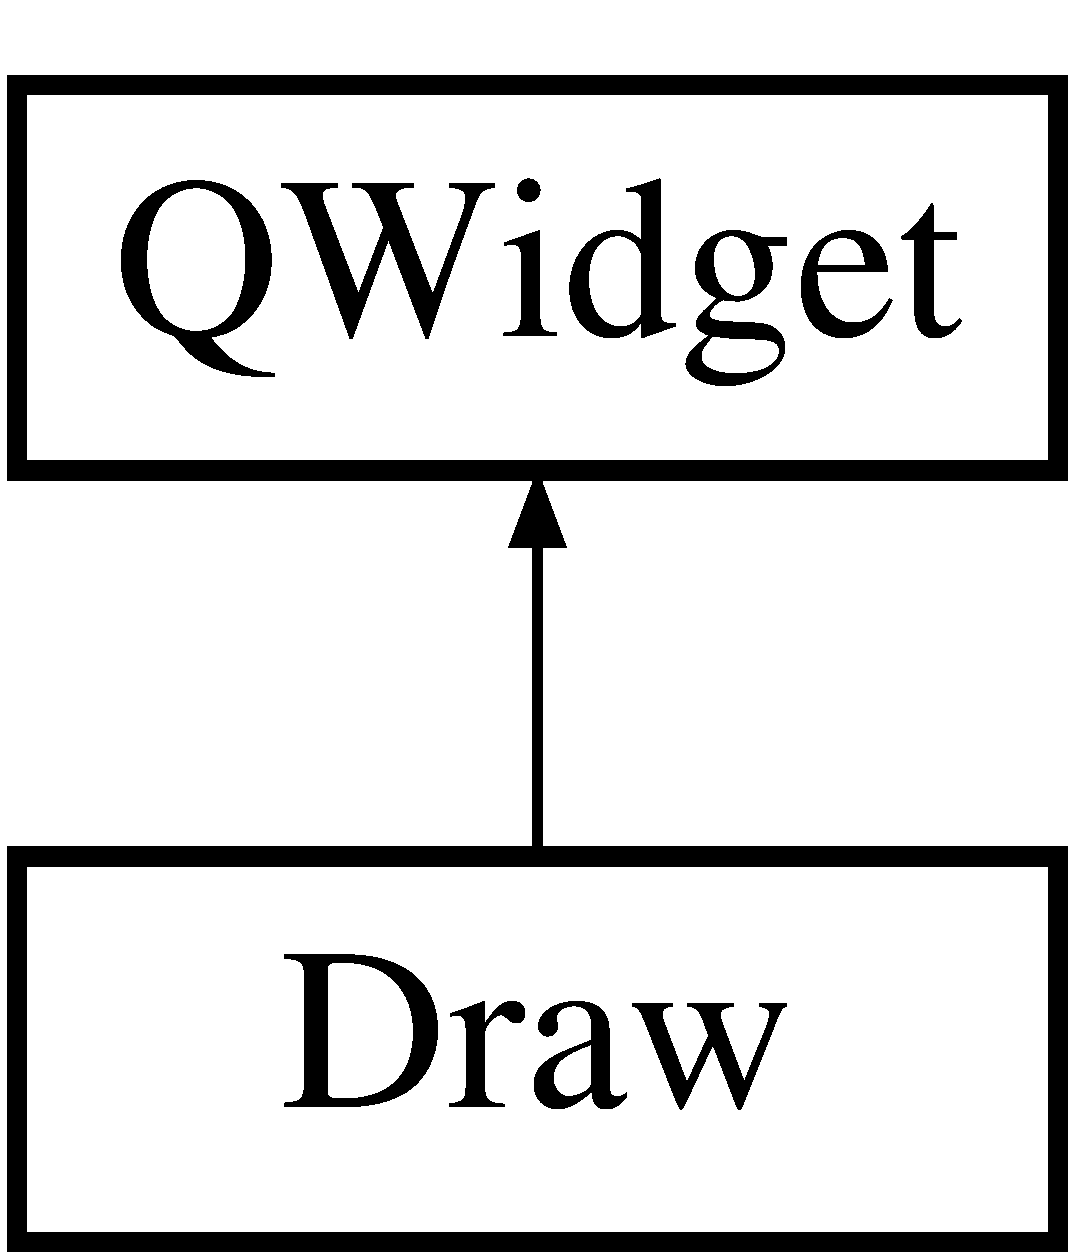
\includegraphics[height=2.000000cm]{class_draw}
\end{center}
\end{figure}
\subsection*{Public Slots}
\begin{DoxyCompactItemize}
\item 
\hypertarget{class_draw_a4e01f0c9c841a83b86cee5f35b4041a2}{}int \hyperlink{class_draw_a4e01f0c9c841a83b86cee5f35b4041a2}{fps} ()\label{class_draw_a4e01f0c9c841a83b86cee5f35b4041a2}

\begin{DoxyCompactList}\small\item\em Wird angetriggert wenn die fps angezeigt wird. \end{DoxyCompactList}\item 
\hypertarget{class_draw_a706414ad08bb093ccd2bcd61e12dabe1}{}void \hyperlink{class_draw_a706414ad08bb093ccd2bcd61e12dabe1}{win\+C} ()\label{class_draw_a706414ad08bb093ccd2bcd61e12dabe1}

\begin{DoxyCompactList}\small\item\em Wird angetriggert wenn der erste Spieler gewinnt. \end{DoxyCompactList}\item 
\hypertarget{class_draw_ac63e4e142c5a594016d51a80f7de5194}{}void \hyperlink{class_draw_ac63e4e142c5a594016d51a80f7de5194}{win\+E} ()\label{class_draw_ac63e4e142c5a594016d51a80f7de5194}

\begin{DoxyCompactList}\small\item\em Wird angetriggert wenn der zweite Spieler/\+K\+I gewinnt. \end{DoxyCompactList}\item 
void \hyperlink{class_draw_a16841fa2b2ccda01f1e90d657d4427bc}{ki\+Action\+True} ()
\begin{DoxyCompactList}\small\item\em Wird angetriggert wenn die K\+I wieder einen Zug machen soll. \end{DoxyCompactList}\end{DoxyCompactItemize}
\subsection*{Signals}
\begin{DoxyCompactItemize}
\item 
void \hyperlink{class_draw_af9ed50b9ec6a3bae6a995a394e6c58e3}{chat\+Signal} ()
\begin{DoxyCompactList}\small\item\em Signalisiert dem \hyperlink{class_chat}{Chat} das er versteckt oder angezeigt werden soll. \end{DoxyCompactList}\item 
void \hyperlink{class_draw_ad2ba543f075871b08e4fb22bcfa00a7f}{show\+Only\+Chat} ()
\begin{DoxyCompactList}\small\item\em Zeigt nur den \hyperlink{class_chat}{Chat}. \end{DoxyCompactList}\item 
void \hyperlink{class_draw_a799aeae3d852fe42b9521f6cef53c41e}{hide\+Only\+Chat} ()
\begin{DoxyCompactList}\small\item\em Versteckt nur den \hyperlink{class_chat}{Chat}. \end{DoxyCompactList}\item 
void \hyperlink{class_draw_a8e1664e9a5bdb18ddfedfe8cbc7e9de3}{set\+Current} (int)
\begin{DoxyCompactList}\small\item\em Signalisiert der Main das ein anderes Widget angezeigt werden soll. \end{DoxyCompactList}\end{DoxyCompactItemize}
\subsection*{Public Member Functions}
\begin{DoxyCompactItemize}
\item 
\hyperlink{class_draw_a04439e9d5f430ebe2c1cf8216b542930}{Draw} (Q\+Widget $\ast$parent=0)
\begin{DoxyCompactList}\small\item\em Constructor der Klasse \hyperlink{class_draw}{Draw}. \end{DoxyCompactList}\item 
void \hyperlink{class_draw_a2db5297d01a7a230a1e5a504e22e4b1a}{set\+Fps\+Visible} (bool b)
\begin{DoxyCompactList}\small\item\em Setzt die Fps sichtbar. \end{DoxyCompactList}\item 
bool \hyperlink{class_draw_a70803e861847ba4d1fce021502eb9d2b}{is\+Fps\+Visible} ()
\begin{DoxyCompactList}\small\item\em Gibt an ob die Fps sichtbar sind. \end{DoxyCompactList}\item 
void \hyperlink{class_draw_a14d84222a5d90e9061d5a46ccfae2539}{load} (int sel\+Char, int sel\+Backg, int sel\+Char2)
\begin{DoxyCompactList}\small\item\em Ladet die gewählten Charaktere und den Hintergrund. \end{DoxyCompactList}\end{DoxyCompactItemize}
\subsection*{Protected Member Functions}
\begin{DoxyCompactItemize}
\item 
void \hyperlink{class_draw_ae94babea5ece40d00e4c8e5e0b5506e7}{paint\+Event} (Q\+Paint\+Event $\ast$e)
\begin{DoxyCompactList}\small\item\em Zeichnet Elemente für die Klasse. \end{DoxyCompactList}\item 
void \hyperlink{class_draw_a6d1346ffb671cc8e622700125b0dbc60}{key\+Press\+Event} (Q\+Key\+Event $\ast$e)
\begin{DoxyCompactList}\small\item\em Registriert die Tastenschläge des Benutzers. \end{DoxyCompactList}\item 
void \hyperlink{class_draw_a9aff693268ed2232fbb4154617ea49cc}{key\+Release\+Event} (Q\+Key\+Event $\ast$e)
\begin{DoxyCompactList}\small\item\em Registriert wenn der Benutzer die Taste loslässt. \end{DoxyCompactList}\end{DoxyCompactItemize}


\subsection{Detailed Description}
Die \hyperlink{class_draw}{Draw} Klasse (ruft die Klassen \hyperlink{class_character}{Character}, \hyperlink{class_background}{Background} und Ui\+Overlay auf). 

Die Klasse \hyperlink{class_draw}{Draw} ruft die Klassen \hyperlink{class_character}{Character}, \hyperlink{class_background}{Background} und Ui\+Overlay auf. Diese sind für das Zeichnen im Spiel verantwortlich. \hyperlink{class_character}{Character} und \hyperlink{class_background}{Background} werden Zahlen übergeben welche für die jeweilige Auswahl stehen (\hyperlink{class_background}{Background} 1, 2, ... etc.). Die Ui\+Overlay Klasse brauch zum Zeichnen immer den \hyperlink{class_character}{Character} als object, damit Healthbar etc. korrekte Werte zeichnen. 

Definition at line 21 of file draw.\+h.



\subsection{Constructor \& Destructor Documentation}
\hypertarget{class_draw_a04439e9d5f430ebe2c1cf8216b542930}{}\index{Draw@{Draw}!Draw@{Draw}}
\index{Draw@{Draw}!Draw@{Draw}}
\subsubsection[{Draw}]{\setlength{\rightskip}{0pt plus 5cm}Draw\+::\+Draw (
\begin{DoxyParamCaption}
\item[{Q\+Widget $\ast$}]{parent = {\ttfamily 0}}
\end{DoxyParamCaption}
)\hspace{0.3cm}{\ttfamily [explicit]}}\label{class_draw_a04439e9d5f430ebe2c1cf8216b542930}


Constructor der Klasse \hyperlink{class_draw}{Draw}. 

Contructor der Klasse \hyperlink{class_draw}{Draw}. 
\begin{DoxyParams}{Parameters}
{\em parent} & Übergibt falls vorhanden das parent-\/\+Q\+Widget. \\
\hline
\end{DoxyParams}


Definition at line 3 of file draw.\+cpp.



\subsection{Member Function Documentation}
\hypertarget{class_draw_af9ed50b9ec6a3bae6a995a394e6c58e3}{}\index{Draw@{Draw}!chat\+Signal@{chat\+Signal}}
\index{chat\+Signal@{chat\+Signal}!Draw@{Draw}}
\subsubsection[{chat\+Signal}]{\setlength{\rightskip}{0pt plus 5cm}void Draw\+::chat\+Signal (
\begin{DoxyParamCaption}
{}
\end{DoxyParamCaption}
)\hspace{0.3cm}{\ttfamily [signal]}}\label{class_draw_af9ed50b9ec6a3bae6a995a394e6c58e3}


Signalisiert dem \hyperlink{class_chat}{Chat} das er versteckt oder angezeigt werden soll. 

chat\+Signal \hypertarget{class_draw_a799aeae3d852fe42b9521f6cef53c41e}{}\index{Draw@{Draw}!hide\+Only\+Chat@{hide\+Only\+Chat}}
\index{hide\+Only\+Chat@{hide\+Only\+Chat}!Draw@{Draw}}
\subsubsection[{hide\+Only\+Chat}]{\setlength{\rightskip}{0pt plus 5cm}void Draw\+::hide\+Only\+Chat (
\begin{DoxyParamCaption}
{}
\end{DoxyParamCaption}
)\hspace{0.3cm}{\ttfamily [signal]}}\label{class_draw_a799aeae3d852fe42b9521f6cef53c41e}


Versteckt nur den \hyperlink{class_chat}{Chat}. 

hide\+Only\+Chat \hypertarget{class_draw_a70803e861847ba4d1fce021502eb9d2b}{}\index{Draw@{Draw}!is\+Fps\+Visible@{is\+Fps\+Visible}}
\index{is\+Fps\+Visible@{is\+Fps\+Visible}!Draw@{Draw}}
\subsubsection[{is\+Fps\+Visible}]{\setlength{\rightskip}{0pt plus 5cm}bool Draw\+::is\+Fps\+Visible (
\begin{DoxyParamCaption}
{}
\end{DoxyParamCaption}
)}\label{class_draw_a70803e861847ba4d1fce021502eb9d2b}


Gibt an ob die Fps sichtbar sind. 

is\+Fps\+Visible \begin{DoxyReturn}{Returns}
show\+Fps 
\end{DoxyReturn}


Definition at line 127 of file draw.\+cpp.

\hypertarget{class_draw_a6d1346ffb671cc8e622700125b0dbc60}{}\index{Draw@{Draw}!key\+Press\+Event@{key\+Press\+Event}}
\index{key\+Press\+Event@{key\+Press\+Event}!Draw@{Draw}}
\subsubsection[{key\+Press\+Event}]{\setlength{\rightskip}{0pt plus 5cm}void Draw\+::key\+Press\+Event (
\begin{DoxyParamCaption}
\item[{Q\+Key\+Event $\ast$}]{e}
\end{DoxyParamCaption}
)\hspace{0.3cm}{\ttfamily [protected]}}\label{class_draw_a6d1346ffb671cc8e622700125b0dbc60}


Registriert die Tastenschläge des Benutzers. 

key\+Press\+Event 
\begin{DoxyParams}{Parameters}
{\em e} & Die Taste welche gedrückt wird. \\
\hline
\end{DoxyParams}


Definition at line 131 of file draw.\+cpp.

\hypertarget{class_draw_a9aff693268ed2232fbb4154617ea49cc}{}\index{Draw@{Draw}!key\+Release\+Event@{key\+Release\+Event}}
\index{key\+Release\+Event@{key\+Release\+Event}!Draw@{Draw}}
\subsubsection[{key\+Release\+Event}]{\setlength{\rightskip}{0pt plus 5cm}void Draw\+::key\+Release\+Event (
\begin{DoxyParamCaption}
\item[{Q\+Key\+Event $\ast$}]{e}
\end{DoxyParamCaption}
)\hspace{0.3cm}{\ttfamily [protected]}}\label{class_draw_a9aff693268ed2232fbb4154617ea49cc}


Registriert wenn der Benutzer die Taste loslässt. 

key\+Release\+Event 
\begin{DoxyParams}{Parameters}
{\em e} & Die Taste welche losgelassen wurde. \\
\hline
\end{DoxyParams}


Definition at line 185 of file draw.\+cpp.

\hypertarget{class_draw_a16841fa2b2ccda01f1e90d657d4427bc}{}\index{Draw@{Draw}!ki\+Action\+True@{ki\+Action\+True}}
\index{ki\+Action\+True@{ki\+Action\+True}!Draw@{Draw}}
\subsubsection[{ki\+Action\+True}]{\setlength{\rightskip}{0pt plus 5cm}void Draw\+::ki\+Action\+True (
\begin{DoxyParamCaption}
{}
\end{DoxyParamCaption}
)\hspace{0.3cm}{\ttfamily [slot]}}\label{class_draw_a16841fa2b2ccda01f1e90d657d4427bc}


Wird angetriggert wenn die K\+I wieder einen Zug machen soll. 

\hyperlink{class_draw_a16841fa2b2ccda01f1e90d657d4427bc}{Draw\+::ki\+Action\+True}.

Setzt die K\+I Action true sodass die K\+I beim nächsten Zug wieder eine Aktion machen soll. 

Definition at line 283 of file draw.\+cpp.

\hypertarget{class_draw_a14d84222a5d90e9061d5a46ccfae2539}{}\index{Draw@{Draw}!load@{load}}
\index{load@{load}!Draw@{Draw}}
\subsubsection[{load}]{\setlength{\rightskip}{0pt plus 5cm}void Draw\+::load (
\begin{DoxyParamCaption}
\item[{int}]{sel\+Char, }
\item[{int}]{sel\+Backg, }
\item[{int}]{sel\+Char2}
\end{DoxyParamCaption}
)}\label{class_draw_a14d84222a5d90e9061d5a46ccfae2539}


Ladet die gewählten Charaktere und den Hintergrund. 

load 
\begin{DoxyParams}{Parameters}
{\em sel\+Char} & der gewählte Charakter. \\
\hline
{\em sel\+Backg} & der gewählte Hintergrund. \\
\hline
{\em sel\+Char2} & der gewählte 2.\+Charakter. \\
\hline
\end{DoxyParams}


Definition at line 219 of file draw.\+cpp.

\hypertarget{class_draw_ae94babea5ece40d00e4c8e5e0b5506e7}{}\index{Draw@{Draw}!paint\+Event@{paint\+Event}}
\index{paint\+Event@{paint\+Event}!Draw@{Draw}}
\subsubsection[{paint\+Event}]{\setlength{\rightskip}{0pt plus 5cm}void Draw\+::paint\+Event (
\begin{DoxyParamCaption}
\item[{Q\+Paint\+Event $\ast$}]{e}
\end{DoxyParamCaption}
)\hspace{0.3cm}{\ttfamily [protected]}}\label{class_draw_ae94babea5ece40d00e4c8e5e0b5506e7}


Zeichnet Elemente für die Klasse. 

paint\+Event 
\begin{DoxyParams}{Parameters}
{\em e} & Das paint\+Event. \\
\hline
\end{DoxyParams}


Definition at line 36 of file draw.\+cpp.

\hypertarget{class_draw_a8e1664e9a5bdb18ddfedfe8cbc7e9de3}{}\index{Draw@{Draw}!set\+Current@{set\+Current}}
\index{set\+Current@{set\+Current}!Draw@{Draw}}
\subsubsection[{set\+Current}]{\setlength{\rightskip}{0pt plus 5cm}void Draw\+::set\+Current (
\begin{DoxyParamCaption}
\item[{int}]{}
\end{DoxyParamCaption}
)\hspace{0.3cm}{\ttfamily [signal]}}\label{class_draw_a8e1664e9a5bdb18ddfedfe8cbc7e9de3}


Signalisiert der Main das ein anderes Widget angezeigt werden soll. 

set\+Current 
\begin{DoxyParams}{Parameters}
{\em int} & Das Widget welches angezeigt werden soll. \\
\hline
\end{DoxyParams}
\hypertarget{class_draw_a2db5297d01a7a230a1e5a504e22e4b1a}{}\index{Draw@{Draw}!set\+Fps\+Visible@{set\+Fps\+Visible}}
\index{set\+Fps\+Visible@{set\+Fps\+Visible}!Draw@{Draw}}
\subsubsection[{set\+Fps\+Visible}]{\setlength{\rightskip}{0pt plus 5cm}void Draw\+::set\+Fps\+Visible (
\begin{DoxyParamCaption}
\item[{bool}]{b}
\end{DoxyParamCaption}
)}\label{class_draw_a2db5297d01a7a230a1e5a504e22e4b1a}


Setzt die Fps sichtbar. 

set\+Fps\+Visible 
\begin{DoxyParams}{Parameters}
{\em b} & True -\/ Fps ist sichtbar.~\newline
False -\/ Fps nicht sichtbar. \\
\hline
\end{DoxyParams}


Definition at line 123 of file draw.\+cpp.

\hypertarget{class_draw_ad2ba543f075871b08e4fb22bcfa00a7f}{}\index{Draw@{Draw}!show\+Only\+Chat@{show\+Only\+Chat}}
\index{show\+Only\+Chat@{show\+Only\+Chat}!Draw@{Draw}}
\subsubsection[{show\+Only\+Chat}]{\setlength{\rightskip}{0pt plus 5cm}void Draw\+::show\+Only\+Chat (
\begin{DoxyParamCaption}
{}
\end{DoxyParamCaption}
)\hspace{0.3cm}{\ttfamily [signal]}}\label{class_draw_ad2ba543f075871b08e4fb22bcfa00a7f}


Zeigt nur den \hyperlink{class_chat}{Chat}. 

show\+Only\+Chat 

The documentation for this class was generated from the following files\+:\begin{DoxyCompactItemize}
\item 
draw.\+h\item 
draw.\+cpp\end{DoxyCompactItemize}

\hypertarget{class_draw_object}{}\section{Draw\+Object Class Reference}
\label{class_draw_object}\index{Draw\+Object@{Draw\+Object}}


draw\+Object Klasse um ein Objekt zeichnen zu können.  




{\ttfamily \#include $<$drawobject.\+h$>$}

Inheritance diagram for Draw\+Object\+:\begin{figure}[H]
\begin{center}
\leavevmode
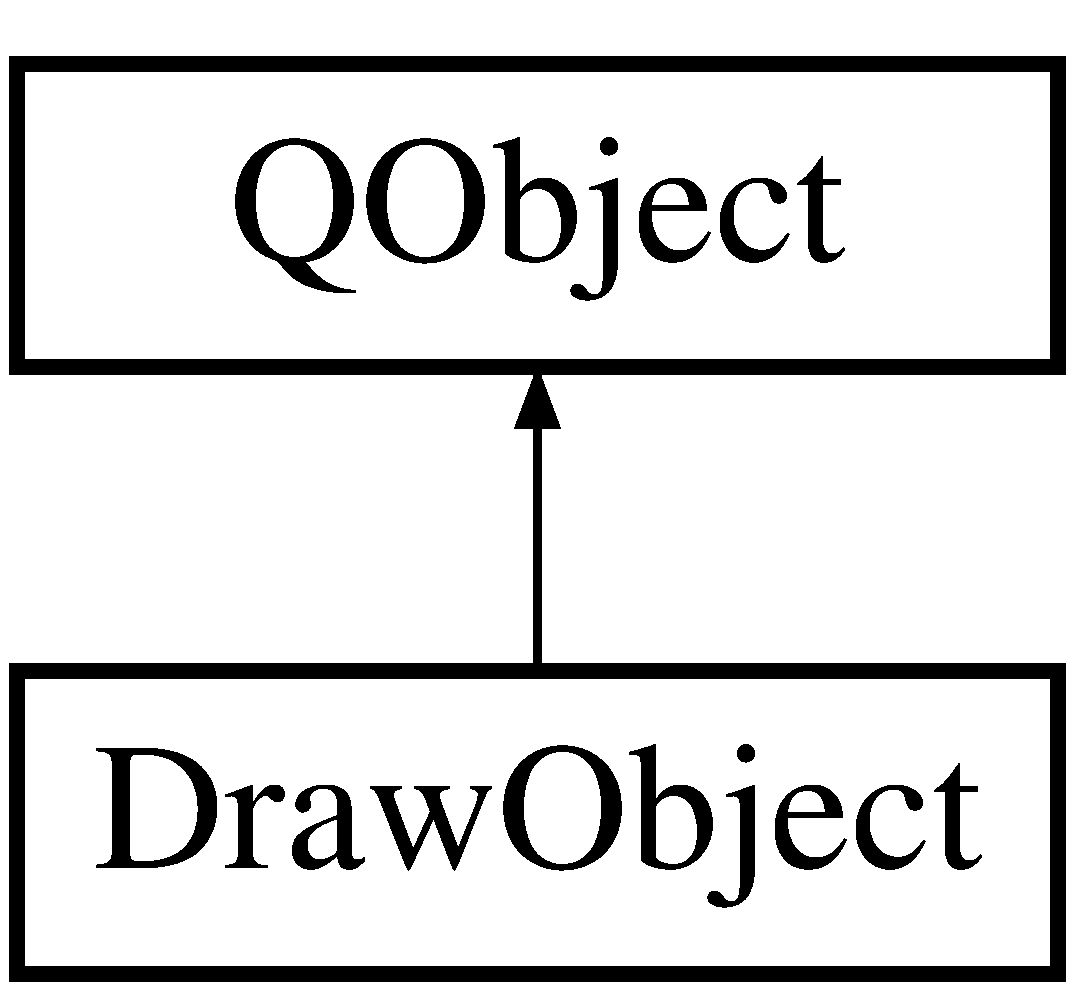
\includegraphics[height=2.000000cm]{class_draw_object}
\end{center}
\end{figure}
\subsection*{Public Slots}
\begin{DoxyCompactItemize}
\item 
Q\+Image \hyperlink{class_draw_object_aa32cf1d16d28633a145dcf28c899a9f2}{get\+Object} ()
\begin{DoxyCompactList}\small\item\em Gibt ein Objekt/\+Frame zurück. \end{DoxyCompactList}\end{DoxyCompactItemize}
\subsection*{Public Member Functions}
\begin{DoxyCompactItemize}
\item 
\hyperlink{class_draw_object_ad2957b36afe08d84a3a4b5de876cac30}{Draw\+Object} (Q\+String source, int \+\_\+frame\+X, int \+\_\+frame\+Y, Q\+Object $\ast$parent=0)
\begin{DoxyCompactList}\small\item\em Contructor der draw\+Object Klasse. \end{DoxyCompactList}\end{DoxyCompactItemize}


\subsection{Detailed Description}
draw\+Object Klasse um ein Objekt zeichnen zu können. 

\subsection{Constructor \& Destructor Documentation}
\hypertarget{class_draw_object_ad2957b36afe08d84a3a4b5de876cac30}{}\index{Draw\+Object@{Draw\+Object}!Draw\+Object@{Draw\+Object}}
\index{Draw\+Object@{Draw\+Object}!Draw\+Object@{Draw\+Object}}
\subsubsection[{Draw\+Object}]{\setlength{\rightskip}{0pt plus 5cm}Draw\+Object\+::\+Draw\+Object (
\begin{DoxyParamCaption}
\item[{Q\+String}]{source, }
\item[{int}]{\+\_\+frame\+X, }
\item[{int}]{\+\_\+frame\+Y, }
\item[{Q\+Object $\ast$}]{parent = {\ttfamily 0}}
\end{DoxyParamCaption}
)\hspace{0.3cm}{\ttfamily [explicit]}}\label{class_draw_object_ad2957b36afe08d84a3a4b5de876cac30}


Contructor der draw\+Object Klasse. 

Constructor der Klasse \hyperlink{class_draw_object}{Draw\+Object}. 
\begin{DoxyParams}{Parameters}
{\em source} & Die Quelle des Frames. \\
\hline
{\em \+\_\+frame\+X} & X-\/\+Wert des Frames. \\
\hline
{\em \+\_\+frame\+Y} & Y-\/\+Wert des Frames. \\
\hline
{\em parent} & Das parent Widget falls vorhanden. \\
\hline
\end{DoxyParams}


\subsection{Member Function Documentation}
\hypertarget{class_draw_object_aa32cf1d16d28633a145dcf28c899a9f2}{}\index{Draw\+Object@{Draw\+Object}!get\+Object@{get\+Object}}
\index{get\+Object@{get\+Object}!Draw\+Object@{Draw\+Object}}
\subsubsection[{get\+Object}]{\setlength{\rightskip}{0pt plus 5cm}Q\+Image Draw\+Object\+::get\+Object (
\begin{DoxyParamCaption}
{}
\end{DoxyParamCaption}
)\hspace{0.3cm}{\ttfamily [slot]}}\label{class_draw_object_aa32cf1d16d28633a145dcf28c899a9f2}


Gibt ein Objekt/\+Frame zurück. 

get\+Object \begin{DoxyReturn}{Returns}
Das erstellte Bild 
\end{DoxyReturn}


The documentation for this class was generated from the following files\+:\begin{DoxyCompactItemize}
\item 
drawobject.\+h\item 
drawobject.\+cpp\end{DoxyCompactItemize}

\hypertarget{class_fighterino}{}\section{Fighterino Class Reference}
\label{class_fighterino}\index{Fighterino@{Fighterino}}


\hyperlink{class_fighterino}{Fighterino} Klasse für die Menüs.  




{\ttfamily \#include $<$fighterino.\+h$>$}

Inheritance diagram for Fighterino\+:\begin{figure}[H]
\begin{center}
\leavevmode
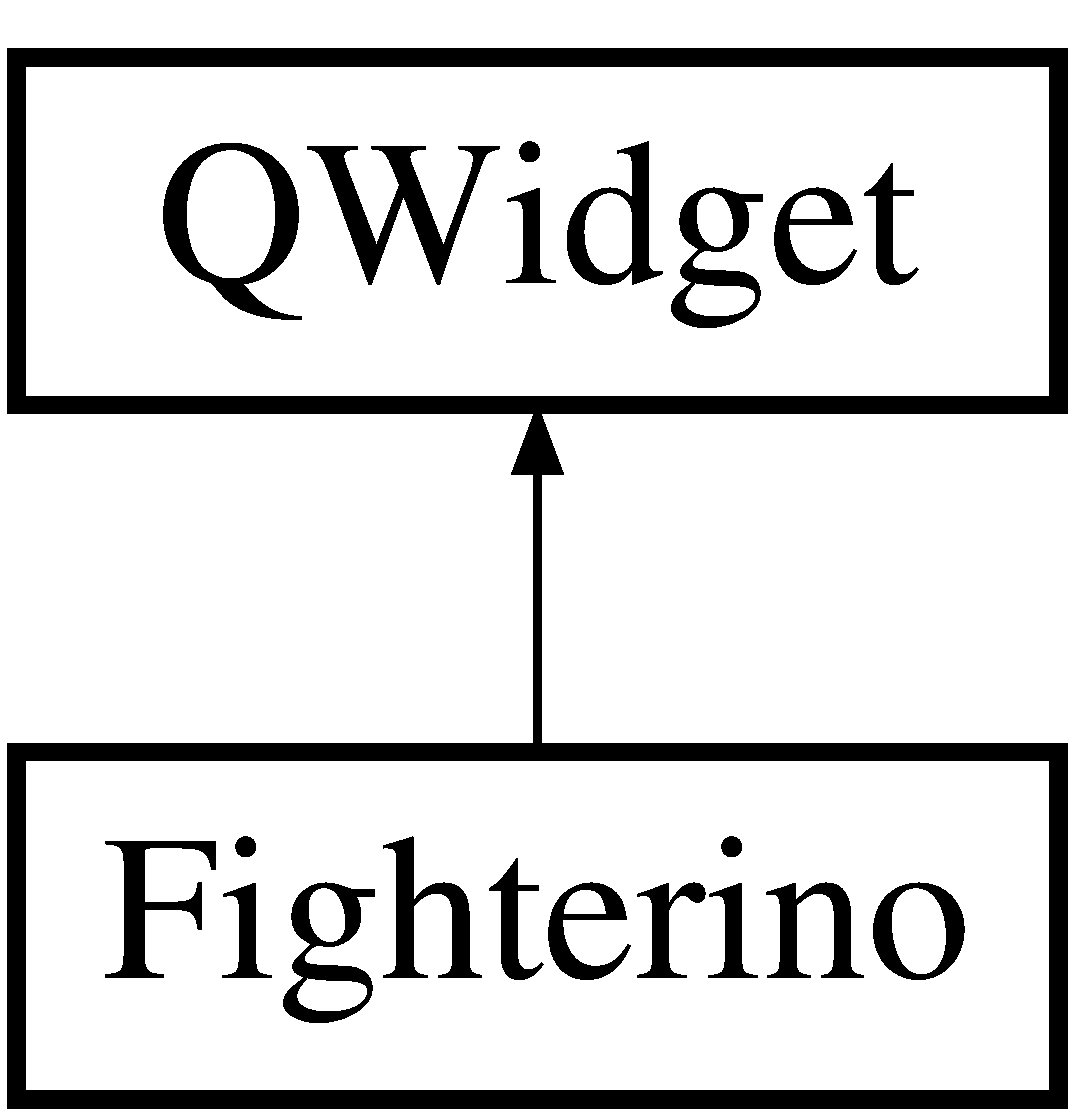
\includegraphics[height=2.000000cm]{class_fighterino}
\end{center}
\end{figure}
\subsection*{Public Member Functions}
\begin{DoxyCompactItemize}
\item 
\hyperlink{class_fighterino_a133b36eb3731d07d14262c9043f536eb}{Fighterino} (Q\+Widget $\ast$parent=0)
\begin{DoxyCompactList}\small\item\em der \hyperlink{class_fighterino}{Fighterino} Constructor. \end{DoxyCompactList}\end{DoxyCompactItemize}
\subsection*{Protected Member Functions}
\begin{DoxyCompactItemize}
\item 
void \hyperlink{class_fighterino_a59266485815dfc7e13c5cbb0ab3310a8}{key\+Press\+Event} (Q\+Key\+Event $\ast$e)
\begin{DoxyCompactList}\small\item\em Registriert die Tastenschläge des Benutzers. \end{DoxyCompactList}\item 
void \hyperlink{class_fighterino_aa8a42ffd3f2794c406f7d7e80cb45bfd}{resize\+Event} (Q\+Resize\+Event $\ast$event)
\begin{DoxyCompactList}\small\item\em Erhält Widgets Größenveränderung-\/\+Ereignisse, die in dem Event-\/\+Parameter übergeben werden. \end{DoxyCompactList}\end{DoxyCompactItemize}


\subsection{Detailed Description}
\hyperlink{class_fighterino}{Fighterino} Klasse für die Menüs. 

Diese Klasse liefert die Widgets für die Menüs und Auswahlmöglichkeiten. 

\subsection{Constructor \& Destructor Documentation}
\hypertarget{class_fighterino_a133b36eb3731d07d14262c9043f536eb}{}\index{Fighterino@{Fighterino}!Fighterino@{Fighterino}}
\index{Fighterino@{Fighterino}!Fighterino@{Fighterino}}
\subsubsection[{Fighterino}]{\setlength{\rightskip}{0pt plus 5cm}Fighterino\+::\+Fighterino (
\begin{DoxyParamCaption}
\item[{Q\+Widget $\ast$}]{parent = {\ttfamily 0}}
\end{DoxyParamCaption}
)\hspace{0.3cm}{\ttfamily [explicit]}}\label{class_fighterino_a133b36eb3731d07d14262c9043f536eb}


der \hyperlink{class_fighterino}{Fighterino} Constructor. 

Contructor der Klasse \hyperlink{class_fighterino}{Fighterino}. 
\begin{DoxyParams}{Parameters}
{\em parent} & Übergibt falls vorhanden das parent-\/\+Q\+Widget. \\
\hline
\end{DoxyParams}


\subsection{Member Function Documentation}
\hypertarget{class_fighterino_a59266485815dfc7e13c5cbb0ab3310a8}{}\index{Fighterino@{Fighterino}!key\+Press\+Event@{key\+Press\+Event}}
\index{key\+Press\+Event@{key\+Press\+Event}!Fighterino@{Fighterino}}
\subsubsection[{key\+Press\+Event}]{\setlength{\rightskip}{0pt plus 5cm}void Fighterino\+::key\+Press\+Event (
\begin{DoxyParamCaption}
\item[{Q\+Key\+Event $\ast$}]{e}
\end{DoxyParamCaption}
)\hspace{0.3cm}{\ttfamily [protected]}}\label{class_fighterino_a59266485815dfc7e13c5cbb0ab3310a8}


Registriert die Tastenschläge des Benutzers. 

key\+Press\+Event 
\begin{DoxyParams}{Parameters}
{\em e} & Die Taste welche gedrückt wird. \\
\hline
\end{DoxyParams}
\hypertarget{class_fighterino_aa8a42ffd3f2794c406f7d7e80cb45bfd}{}\index{Fighterino@{Fighterino}!resize\+Event@{resize\+Event}}
\index{resize\+Event@{resize\+Event}!Fighterino@{Fighterino}}
\subsubsection[{resize\+Event}]{\setlength{\rightskip}{0pt plus 5cm}void Fighterino\+::resize\+Event (
\begin{DoxyParamCaption}
\item[{Q\+Resize\+Event $\ast$}]{event}
\end{DoxyParamCaption}
)\hspace{0.3cm}{\ttfamily [protected]}}\label{class_fighterino_aa8a42ffd3f2794c406f7d7e80cb45bfd}


Erhält Widgets Größenveränderung-\/\+Ereignisse, die in dem Event-\/\+Parameter übergeben werden. 

resize\+Event 
\begin{DoxyParams}{Parameters}
{\em event} & Das Resize\+Event. \\
\hline
\end{DoxyParams}


The documentation for this class was generated from the following files\+:\begin{DoxyCompactItemize}
\item 
fighterino.\+h\item 
fighterino.\+cpp\end{DoxyCompactItemize}

\hypertarget{class_sprite}{}\section{Sprite Class Reference}
\label{class_sprite}\index{Sprite@{Sprite}}
\subsection*{Public Member Functions}
\begin{DoxyCompactItemize}
\item 
\hypertarget{class_sprite_a247eff7723c39ee82ba183e975f644dd}{}{\bfseries Sprite} (Q\+Image bild)\label{class_sprite_a247eff7723c39ee82ba183e975f644dd}

\item 
\hypertarget{class_sprite_a37b20fb41171754d6cc893a1efe9cea8}{}Q\+Image {\bfseries get\+Image} ()\label{class_sprite_a37b20fb41171754d6cc893a1efe9cea8}

\item 
\hypertarget{class_sprite_ad225df2276134a2374a2e6a751a9beeb}{}Q\+Image {\bfseries get\+Image} (int sequence)\label{class_sprite_ad225df2276134a2374a2e6a751a9beeb}

\item 
\hypertarget{class_sprite_a791c9dfd90379dfcc2466b0049b41967}{}Q\+Image {\bfseries get\+Image\+Mirrored} (int sequence)\label{class_sprite_a791c9dfd90379dfcc2466b0049b41967}

\item 
Q\+Image \hyperlink{class_sprite_abd18da77e4c85a62bbbcbca6bcf40463}{get\+Image} (int x, int y, int sequence, bool mirrored=false)
\begin{DoxyCompactList}\small\item\em Sprite\+::get\+Image. \end{DoxyCompactList}\end{DoxyCompactItemize}


\subsection{Member Function Documentation}
\hypertarget{class_sprite_abd18da77e4c85a62bbbcbca6bcf40463}{}\index{Sprite@{Sprite}!get\+Image@{get\+Image}}
\index{get\+Image@{get\+Image}!Sprite@{Sprite}}
\subsubsection[{get\+Image}]{\setlength{\rightskip}{0pt plus 5cm}Q\+Image Sprite\+::get\+Image (
\begin{DoxyParamCaption}
\item[{int}]{x, }
\item[{int}]{y, }
\item[{int}]{sequence, }
\item[{bool}]{mirrored = {\ttfamily false}}
\end{DoxyParamCaption}
)}\label{class_sprite_abd18da77e4c85a62bbbcbca6bcf40463}


Sprite\+::get\+Image. 

Diese Funtion bekommt ein sprite$\ast$ image und nimmt die jeweilige


\begin{DoxyParams}{Parameters}
{\em x} & \\
\hline
{\em y} & \\
\hline
{\em sequence} & \\
\hline
{\em mirrored} & \\
\hline
\end{DoxyParams}
\begin{DoxyReturn}{Returns}

\end{DoxyReturn}


The documentation for this class was generated from the following files\+:\begin{DoxyCompactItemize}
\item 
sprite.\+h\item 
sprite.\+cpp\end{DoxyCompactItemize}

\hypertarget{class_start_menu}{}\section{Start\+Menu Class Reference}
\label{class_start_menu}\index{Start\+Menu@{Start\+Menu}}
Inheritance diagram for Start\+Menu\+:\begin{figure}[H]
\begin{center}
\leavevmode
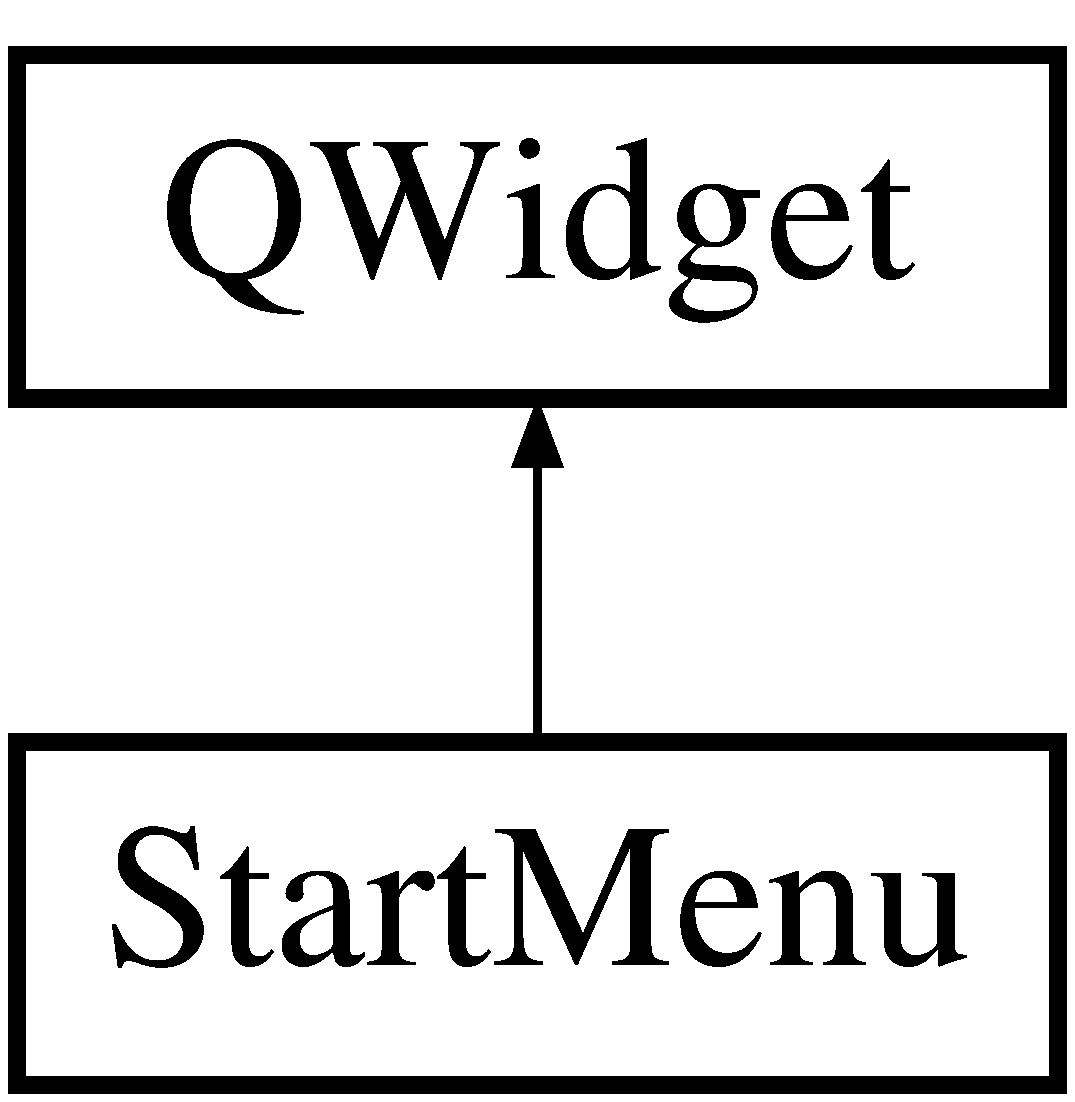
\includegraphics[height=2.000000cm]{class_start_menu}
\end{center}
\end{figure}
\subsection*{Public Slots}
\begin{DoxyCompactItemize}
\item 
void \hyperlink{class_start_menu_a3454310eae3e51ebfcd00b9837e0cd71}{Anim} ()
\begin{DoxyCompactList}\small\item\em Startet die Animation im Start-\/\+Menü. \end{DoxyCompactList}\end{DoxyCompactItemize}
\subsection*{Signals}
\begin{DoxyCompactItemize}
\item 
void \hyperlink{class_start_menu_a5ec52ec6f45dffd4ded1592b4bb9526f}{set\+Current} (int a)
\begin{DoxyCompactList}\small\item\em Signalisiert der Main das ein anderes Widget angezeigt werden soll. \end{DoxyCompactList}\end{DoxyCompactItemize}
\subsection*{Public Member Functions}
\begin{DoxyCompactItemize}
\item 
\hyperlink{class_start_menu_a1491fb2672b951483f3cfc0594571fbb}{Start\+Menu} (Q\+Widget $\ast$parent=0)
\begin{DoxyCompactList}\small\item\em Construktor der Klasse \hyperlink{class_start_menu}{Start\+Menu}. \end{DoxyCompactList}\end{DoxyCompactItemize}
\subsection*{Protected Member Functions}
\begin{DoxyCompactItemize}
\item 
void \hyperlink{class_start_menu_a228c407369ced59d196afd48c1660ed1}{paint\+Event} (Q\+Paint\+Event $\ast$e)
\begin{DoxyCompactList}\small\item\em Zeichnet Elemente für die Klasse. \end{DoxyCompactList}\end{DoxyCompactItemize}
\subsection*{Properties}
\begin{DoxyCompactItemize}
\item 
\hypertarget{class_start_menu_a60a9b0bf69fd27521cef5c8356474f91}{}Q\+Rect {\bfseries ptitle}\label{class_start_menu_a60a9b0bf69fd27521cef5c8356474f91}

\end{DoxyCompactItemize}


\subsection{Constructor \& Destructor Documentation}
\hypertarget{class_start_menu_a1491fb2672b951483f3cfc0594571fbb}{}\index{Start\+Menu@{Start\+Menu}!Start\+Menu@{Start\+Menu}}
\index{Start\+Menu@{Start\+Menu}!Start\+Menu@{Start\+Menu}}
\subsubsection[{Start\+Menu}]{\setlength{\rightskip}{0pt plus 5cm}Start\+Menu\+::\+Start\+Menu (
\begin{DoxyParamCaption}
\item[{Q\+Widget $\ast$}]{parent = {\ttfamily 0}}
\end{DoxyParamCaption}
)\hspace{0.3cm}{\ttfamily [explicit]}}\label{class_start_menu_a1491fb2672b951483f3cfc0594571fbb}


Construktor der Klasse \hyperlink{class_start_menu}{Start\+Menu}. 

\hyperlink{class_start_menu}{Start\+Menu} 
\begin{DoxyParams}{Parameters}
{\em parent} & Das Parent Widget falls vorhanden. \\
\hline
\end{DoxyParams}


\subsection{Member Function Documentation}
\hypertarget{class_start_menu_a3454310eae3e51ebfcd00b9837e0cd71}{}\index{Start\+Menu@{Start\+Menu}!Anim@{Anim}}
\index{Anim@{Anim}!Start\+Menu@{Start\+Menu}}
\subsubsection[{Anim}]{\setlength{\rightskip}{0pt plus 5cm}void Start\+Menu\+::\+Anim (
\begin{DoxyParamCaption}
{}
\end{DoxyParamCaption}
)\hspace{0.3cm}{\ttfamily [slot]}}\label{class_start_menu_a3454310eae3e51ebfcd00b9837e0cd71}


Startet die Animation im Start-\/\+Menü. 

Anim \hypertarget{class_start_menu_a228c407369ced59d196afd48c1660ed1}{}\index{Start\+Menu@{Start\+Menu}!paint\+Event@{paint\+Event}}
\index{paint\+Event@{paint\+Event}!Start\+Menu@{Start\+Menu}}
\subsubsection[{paint\+Event}]{\setlength{\rightskip}{0pt plus 5cm}void Start\+Menu\+::paint\+Event (
\begin{DoxyParamCaption}
\item[{Q\+Paint\+Event $\ast$}]{e}
\end{DoxyParamCaption}
)\hspace{0.3cm}{\ttfamily [protected]}}\label{class_start_menu_a228c407369ced59d196afd48c1660ed1}


Zeichnet Elemente für die Klasse. 

paint\+Event 
\begin{DoxyParams}{Parameters}
{\em e} & Das paint\+Event. \\
\hline
\end{DoxyParams}
\hypertarget{class_start_menu_a5ec52ec6f45dffd4ded1592b4bb9526f}{}\index{Start\+Menu@{Start\+Menu}!set\+Current@{set\+Current}}
\index{set\+Current@{set\+Current}!Start\+Menu@{Start\+Menu}}
\subsubsection[{set\+Current}]{\setlength{\rightskip}{0pt plus 5cm}void Start\+Menu\+::set\+Current (
\begin{DoxyParamCaption}
\item[{int}]{a}
\end{DoxyParamCaption}
)\hspace{0.3cm}{\ttfamily [signal]}}\label{class_start_menu_a5ec52ec6f45dffd4ded1592b4bb9526f}


Signalisiert der Main das ein anderes Widget angezeigt werden soll. 

set\+Current 
\begin{DoxyParams}{Parameters}
{\em a} & Das Widget welches angezeigt werden soll. \\
\hline
\end{DoxyParams}


The documentation for this class was generated from the following files\+:\begin{DoxyCompactItemize}
\item 
startmenu.\+h\item 
startmenu.\+cpp\end{DoxyCompactItemize}

\hypertarget{class_u_i_overlay}{}\section{U\+I\+Overlay Class Reference}
\label{class_u_i_overlay}\index{U\+I\+Overlay@{U\+I\+Overlay}}


\hyperlink{class_u_i_overlay}{U\+I\+Overlay} Klasse ist für die Darstellung des Interfaces zuständig.  




{\ttfamily \#include $<$uioverlay.\+h$>$}

Inheritance diagram for U\+I\+Overlay\+:\begin{figure}[H]
\begin{center}
\leavevmode
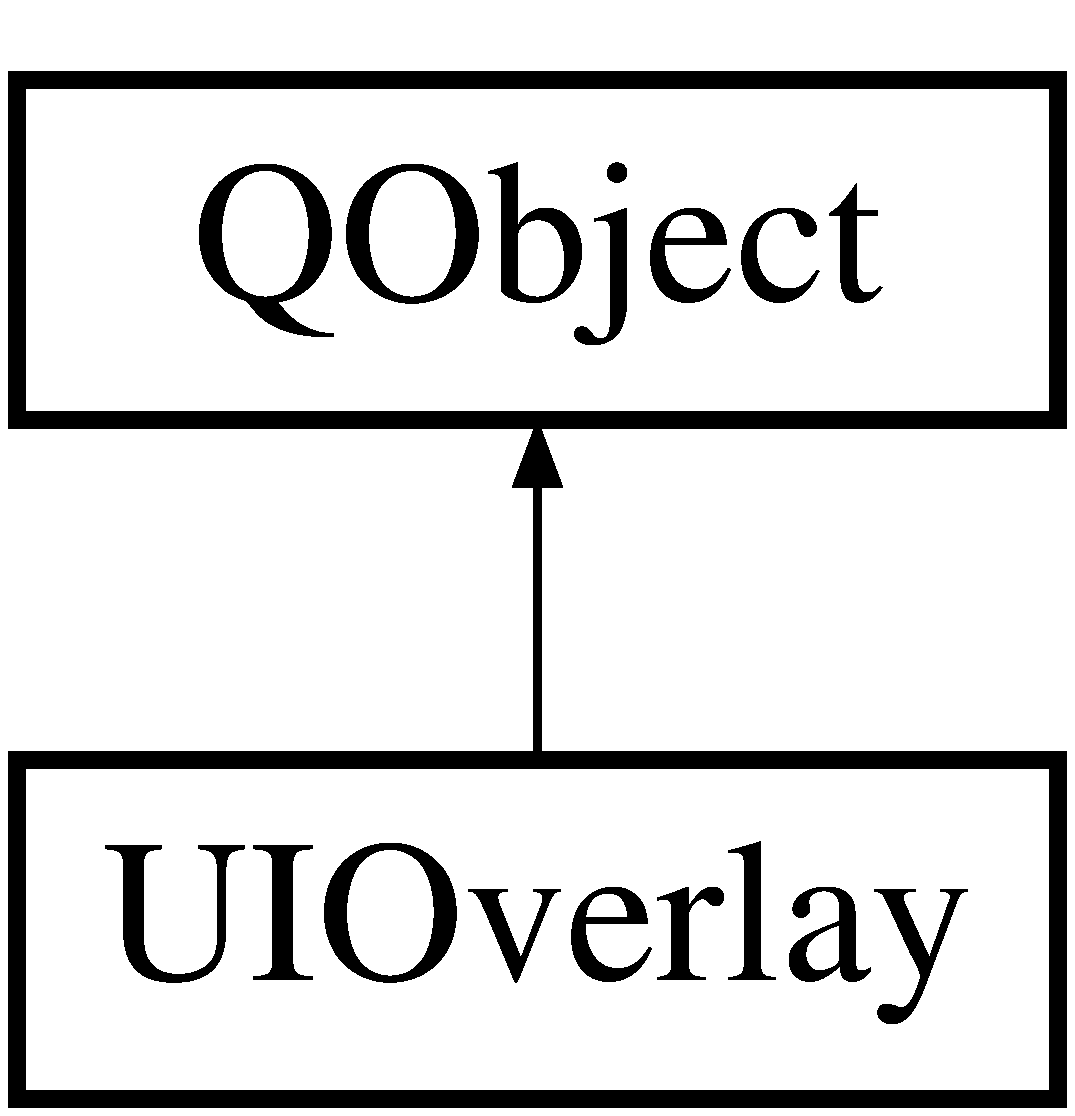
\includegraphics[height=2.000000cm]{class_u_i_overlay}
\end{center}
\end{figure}
\subsection*{Public Slots}
\begin{DoxyCompactItemize}
\item 
void \hyperlink{class_u_i_overlay_a9b3960185a836ecb504ce25d22c1893e}{draw\+Interface} (Q\+Painter $\ast$p, \hyperlink{class_character}{Character} $\ast$c, \hyperlink{class_character}{Character} $\ast$e)
\begin{DoxyCompactList}\small\item\em Zeichnet das Interface. \end{DoxyCompactList}\end{DoxyCompactItemize}
\subsection*{Public Member Functions}
\begin{DoxyCompactItemize}
\item 
\hyperlink{class_u_i_overlay_a51696f81d4333f2c7537a103d9440c47}{U\+I\+Overlay} (Q\+Object $\ast$parent=0)
\begin{DoxyCompactList}\small\item\em Contructor der Klasse \hyperlink{class_u_i_overlay}{U\+I\+Overlay}. \end{DoxyCompactList}\end{DoxyCompactItemize}


\subsection{Detailed Description}
\hyperlink{class_u_i_overlay}{U\+I\+Overlay} Klasse ist für die Darstellung des Interfaces zuständig. 

Hierbei werden die Mana-\/, und Lebensbalken beider Spieler angezeigt. Außerdem gehört zu jedem Spieler ein kleines Profilbild. 

Definition at line 13 of file uioverlay.\+h.



\subsection{Constructor \& Destructor Documentation}
\hypertarget{class_u_i_overlay_a51696f81d4333f2c7537a103d9440c47}{}\index{U\+I\+Overlay@{U\+I\+Overlay}!U\+I\+Overlay@{U\+I\+Overlay}}
\index{U\+I\+Overlay@{U\+I\+Overlay}!U\+I\+Overlay@{U\+I\+Overlay}}
\subsubsection[{U\+I\+Overlay}]{\setlength{\rightskip}{0pt plus 5cm}U\+I\+Overlay\+::\+U\+I\+Overlay (
\begin{DoxyParamCaption}
\item[{Q\+Object $\ast$}]{parent = {\ttfamily 0}}
\end{DoxyParamCaption}
)\hspace{0.3cm}{\ttfamily [explicit]}}\label{class_u_i_overlay_a51696f81d4333f2c7537a103d9440c47}


Contructor der Klasse \hyperlink{class_u_i_overlay}{U\+I\+Overlay}. 

\hyperlink{class_u_i_overlay}{U\+I\+Overlay} Erstellt einige Interface-\/\+Daten. 
\begin{DoxyParams}{Parameters}
{\em parent} & Das parent Widget falls vorhanden. \\
\hline
\end{DoxyParams}


Definition at line 3 of file uioverlay.\+cpp.



\subsection{Member Function Documentation}
\hypertarget{class_u_i_overlay_a9b3960185a836ecb504ce25d22c1893e}{}\index{U\+I\+Overlay@{U\+I\+Overlay}!draw\+Interface@{draw\+Interface}}
\index{draw\+Interface@{draw\+Interface}!U\+I\+Overlay@{U\+I\+Overlay}}
\subsubsection[{draw\+Interface}]{\setlength{\rightskip}{0pt plus 5cm}void U\+I\+Overlay\+::draw\+Interface (
\begin{DoxyParamCaption}
\item[{Q\+Painter $\ast$}]{p, }
\item[{{\bf Character} $\ast$}]{c, }
\item[{{\bf Character} $\ast$}]{e}
\end{DoxyParamCaption}
)\hspace{0.3cm}{\ttfamily [slot]}}\label{class_u_i_overlay_a9b3960185a836ecb504ce25d22c1893e}


Zeichnet das Interface. 

draw\+Interface 
\begin{DoxyParams}{Parameters}
{\em p} & Der Painter damit gezeichnet werden kann. \\
\hline
{\em c} & Informationen vom ersten Spieler. \\
\hline
{\em e} & Informationen vom zweiten Spieler. \\
\hline
\end{DoxyParams}


Definition at line 8 of file uioverlay.\+cpp.



The documentation for this class was generated from the following files\+:\begin{DoxyCompactItemize}
\item 
uioverlay.\+h\item 
uioverlay.\+cpp\end{DoxyCompactItemize}

%--- End generated contents ---

% Index
\backmatter
\newpage
\phantomsection
\clearemptydoublepage
\addcontentsline{toc}{chapter}{Index}
\printindex

\end{document}
